% Training Hyperparameters moved to main text (Section 4)
\section{Dataset Construction}
\label{app:dataset}

Table~\ref{tab:qa_params} lists the QA generation parameters used for constructing FinTSR-Bench.
All tasks use a 120-day input window of daily closing prices.
Assessment tasks evaluate the current state and have no prediction horizon.
For prediction tasks, Event Response and Support/Resistance use a 10-day forward horizon, while Drawdown Recovery, Volatility Forecast, Relative Performance, and Pair Convergence use a 20-day forward horizon.
Table~\ref{tab:class_dist} shows the training set class distribution, confirming that all tasks are approximately balanced via undersampling.


\begin{table}[h]
\centering
\caption{QA generation parameters.}
\label{tab:qa_params}
\vspace{5pt}
\adjustbox{max width=\textwidth}{
\begin{tabular}{ll}
\toprule
\textbf{Parameter} & \textbf{Value} \\
\midrule
Window length & 120 trading days \\
Samples per task (raw) & 100{,}000 \\
Cap per task (train) & 3{,}500 \\
Cap per task (test) & 1{,}000 \\
Correlation thresholds & pos $>$ 0.30, neg $<$ $-$0.10 \\
Event threshold & $|z|$ $>$ 2.5 \\
Rel.\ Perf.\ margin & 5\% \\
Rel.\ Perf.\ forward window & 20 days \\
S/R breakout margin & 3\% \\
Drawdown Recovery min drawdown & 5\% \\
Volatility Forecast change threshold & 25\% \\
Pair Convergence spread margin & 3\% \\
\bottomrule
\end{tabular}
}
\end{table}

\begin{table}[h]
\centering
\caption{\textbf{Training set class distribution.} All tasks are approximately class-balanced via undersampling (3,500 samples per task).}
\label{tab:class_dist}
\vspace{5pt}
\adjustbox{max width=\textwidth}{
\begin{tabular}{l|c|l}
\toprule
\textbf{Task} & \textbf{Classes} & \textbf{Distribution (\%)} \\
\midrule
Drawdown & 4 & A: 24.2, B: 24.3, C: 26.0, D: 25.5 \\
Volatility Regime & 3 & A: 33.5, B: 33.1, C: 33.4 \\
Trend Direction & 5 & A: 20.2, B: 20.4, C: 19.6, D: 21.0, E: 18.7 \\
Correlation & 3 & A: 32.9, B: 34.2, C: 32.9 \\
\midrule
Event Response & 2 & A: 49.0, B: 51.0 \\
Support/Resistance & 2 & A: 50.1, B: 49.9 \\
Drawdown Recovery & 2 & A: 49.0, B: 51.0 \\
Volatility Forecast & 2 & A: 48.9, B: 51.1 \\
Relative Performance & 2 & A: 51.4, B: 48.6 \\
Pair Convergence & 2 & A: 50.5, B: 49.5 \\
\bottomrule
\end{tabular}
}
\end{table}

\clearpage
\textbf{Label construction algorithms.}
We detail the labeling procedure for each prediction task to ensure reproducibility.
\begin{itemize}
\item \textbf{Event Response.} We compute daily returns and their z-scores over the 120-day window. A trading day with $|z| > 2.5$ is flagged as an ``event.'' The label is determined by comparing the 10-day post-event return direction with the event-day return: same direction $\rightarrow$ Persistence, opposite $\rightarrow$ Mean-reversion.
\item \textbf{Support/Resistance.} We identify support (resistance) as the minimum (maximum) closing price over a rolling 60-day lookback window. If the current price is within 5\% of a key level, the sample is included. The label is determined by whether the price moves beyond the level by $>$3\% (Breakout) or stays within it (Bounce) over the next 10 days.
\item \textbf{Drawdown Recovery.} We compute peak price as the running maximum over the window. Stocks with drawdown $>$5\% from peak are included. The label is Recovery if the price moves $>$3\% toward the peak over the next 20 days, and Deepens otherwise.
\item \textbf{Volatility Forecast.} We compute the ratio of 20-day to 120-day return standard deviation. The label is Increase if the 20-day volatility computed at $t{+}20$ exceeds the current 20-day volatility by $>$25\%, and Decrease otherwise.
\item \textbf{Relative Performance.} Given two stocks, the label is determined by which stock achieves a higher cumulative return over the next 20 days. Pairs with $<$5\% return difference are excluded to avoid ambiguous labels.
\item \textbf{Pair Convergence.} We compute the normalized spread as $(P_A - P_B) / (P_A + P_B)$, where $P_A$ and $P_B$ are the closing prices. The label is Convergence if $|\text{spread}_{t+20}| < |\text{spread}_t|$, and Divergence otherwise. Pairs with spread $<$3\% are excluded.
\end{itemize}
To avoid overlapping-window leakage, each task uses a task-specific random seed for sample selection, and we enforce a minimum gap of 20 trading days between consecutive samples from the same stock.

\clearpage
\section{Forecasting Baseline Protocol}
\label{app:forecast_protocol}

All forecasting baselines use the same 120-day input window as FinSTaR and predict over the task-specific horizon (10 or 20 days).
No exogenous covariates are used; all models receive only univariate closing prices.
Predicted price trajectories are converted to classification labels using the same thresholds as the QA generation (e.g., direction of predicted return for Event Response, predicted volatility ratio for Volatility Forecast).

\textbf{Statistical methods} (applied without hyperparameter tuning):
\begin{itemize}
\item \textbf{Last Value.} Predicts the last observed value for all future steps (naive baseline).
\item \textbf{Moving Average (MA).} Predicts the mean of the last $k$ observations ($k{=}20$).
\item \textbf{Exponential Smoothing (ETS)~\cite{ets}.} Weighted average with exponentially decaying weights; captures level and trend.
\item \textbf{Drift.} Extrapolates a linear trend from the first to the last observed value.
\item \textbf{Momentum.} Predicts continuation of the recent return direction over the past 20 days.
\end{itemize}

\textbf{Deep learning models} (trained per-task using AutoGluon TimeSeries with default hyperparameters and early stopping):
\begin{itemize}
\item \textbf{DLinear~\cite{dlinear}.} Decomposes TS into trend and remainder via moving average, then applies linear layers.
\item \textbf{DeepAR~\cite{deepar}.} Autoregressive RNN that produces probabilistic forecasts via learned likelihood parameters.
\item \textbf{PatchTST~\cite{patchtst}.} Patch-based Transformer that segments TS into subseries-level patches for efficient attention.
\item \textbf{TFT~\cite{tft}.} Temporal Fusion Transformer with variable selection, gating, and multi-horizon attention.
\item \textbf{TiDE~\cite{tide}.} MLP-based encoder-decoder with dense residual connections for long-term forecasting.
\end{itemize}

\textbf{Pre-trained forecasting models} (zero-shot, no fine-tuning):
\begin{itemize}
\item \textbf{Chronos-1~\cite{chronos2024}.} Tokenizes TS values into discrete bins and uses a T5-based language model for forecasting.
\item \textbf{Chronos-2~\cite{chronos2024}.} Updated version with improved tokenization and larger pre-training corpus.
\end{itemize}

\clearpage
\section{Scenario Templates}
\label{app:scenario_templates}

Table~\ref{tab:scenario_templates} lists the scenario templates used in Scenario-Aware CoT for all six prediction tasks. For each task and answer, we define three scenarios (base, adverse, favorable) grounded in financial domain knowledge. Assessment tasks (Drawdown, Volatility Regime, Trend Direction, Correlation) use deterministic Compute-in-CoT and do not require scenario templates.

\begin{table}[h]
\centering
\caption{\textbf{Scenario templates for prediction tasks.} Each (task, answer) pair has three domain-specific scenarios.}
\label{tab:scenario_templates}
\vspace{6pt}
\adjustbox{max width=\textwidth}{
\footnotesize
\begin{tabular}{l|l|p{4cm}|p{4cm}|p{4cm}}
\toprule
\textbf{Task} & \textbf{Answer} & \textbf{Base Case} & \textbf{Adverse} & \textbf{Favorable} \\
\midrule
\multirow{4.5}{*}{\textbf{Event Response}} & Mean-reversion & Extreme move partially reverses as market recognizes overreaction & Secondary catalyst reinforces shock direction & Positive news accelerates recovery \\
\cmidrule{2-5}
 & Persistence & Shock reflects genuine new information being priced in & Mean-reversion forces prove it was an overreaction & Additional confirming news amplifies the move \\
\midrule
\multirow{4.5}{*}{\textbf{Support/Resistance}} & Breakout & Price breaks through with sustained momentum & False breakout traps traders, price reverses & High volume accelerates move beyond level \\
\cmidrule{2-5}
 & Bounce & Key level holds as institutional orders defend it & Sustained pressure overwhelms the level & Strong bounce triggers significant reversal \\
\midrule
\multirow{4.5}{*}{\textbf{Drawdown Recovery}} & Recovery & Drawdown stabilizes, value buyers accumulate & Cause worsens (earnings revision, guidance cut) & Positive catalyst triggers V-shaped recovery \\
\cmidrule{2-5}
 & Further decline & Selling pressure continues, drawdown deepens & Surprise positive development reverses decline & Risk-off sentiment compounds weakness \\
\midrule
\multirow{4.5}{*}{\textbf{Volatility Forecast}} & Increase & Volatility clustering continues, uncertainty persists & Uncertainty resolves, volatility collapses & New uncertainty compounds existing volatility \\
\cmidrule{2-5}
 & Decrease & Volatility mean-reverts as shock dissipates & Unexpected event triggers new spike & Broad market calming accelerates compression \\
\midrule
\multirow{4.5}{*}{\textbf{Relative Performance}} & Stock A & Momentum trends persist, Stock A continues trajectory & Stock A headwind, Stock B catalyst reverses gap & Sector tailwinds boost Stock A's advantage \\
\cmidrule{2-5}
 & Stock B & Stock B strengthening continues, Stock A fades & Stock A recovers, re-establishing outperformance & Stock B catalyst (upgrade, M\&A) widens lead \\
\midrule
\multirow{4.5}{*}{\textbf{Pair Convergence}} & Converge & Spread narrows as co-movement reasserts & Structural change sustains divergence & Common catalyst forces rapid convergence \\
\cmidrule{2-5}
 & Diverge & Different fundamentals sustain widening spread & Common catalyst narrows the spread & Company-specific event accelerates divergence \\
\bottomrule
\end{tabular}
}
\end{table}

\clearpage
\section{Full Task Examples}
\label{app:tasks}

We present actual model input, generated CoT reasoning, and output for all ten tasks. Each example shows a correctly predicted sample from Test~A, with the corresponding price series visualization.

\subsection{Assessment Tasks (Compute-in-CoT)}

%%% F1 DRAWDOWN %%%
\begin{figure}[h]
\centering
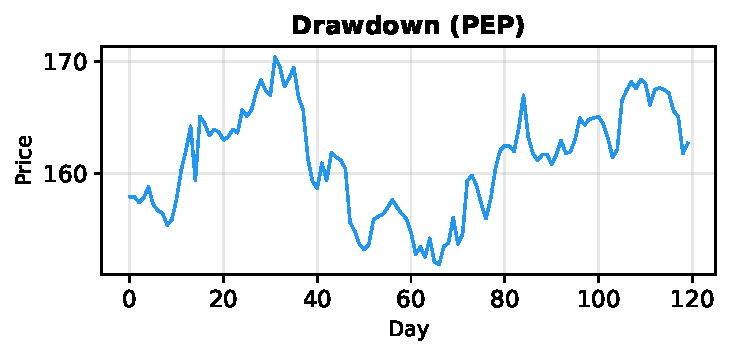
\includegraphics[width=0.95\textwidth]{figures/example_F1_drawdown.pdf}
\vspace{4pt}

\textbf{Task: Drawdown --- Ticker: PEP --- GT: (B) Pullback} \\[4pt]
\begin{minipage}{0.95\textwidth}
\fbox{\parbox{\dimexpr\textwidth-2\fboxsep-2\fboxrule}{
\textbf{Input:} You are analyzing the stock PEP. Below are the daily closing prices for the most recent 120 trading days: [\textit{prices shown above}]. Based on these prices, assess the current drawdown phase. \\
\hspace{6pt}(A) At/Near Peak ($<$3\%) \\
\hspace{6pt}(B) Pullback (3--10\%) \\
\hspace{6pt}(C) Correction (10--20\%) \\
\hspace{6pt}(D) Severe Decline ($>$20\%)
}} \\[4pt]
\fbox{\parbox{\dimexpr\textwidth-2\fboxsep-2\fboxrule}{
\textbf{Output:} \\[6pt]
\texttt{<think>} \\[4pt]
Step 1 --- Find the peak price: \\
Scanning the 120-day series, the highest price is 170.39 (around day 32). \\[6pt]
Step 2 --- Current price: \\
The last price in the series is 162.65. \\[6pt]
Step 3 --- Calculate drawdown: \\
Drawdown = (Peak $-$ Current) / Peak = (170.39 $-$ 162.65) / 170.39 = 4.5\% \\[6pt]
Step 4 --- Classify: \\
4.5\% is between 3\% and 10\%, which corresponds to (B) Pullback. \\[4pt]
\texttt{</think>} \\
\texttt{<answer>(B)</answer>}
}}
\end{minipage}
\caption{(Single-Assessment) Example of Drawdown task.}
\vspace{15pt}
\end{figure}

%%% F2 CORRELATION %%%
\begin{figure}[h]
\centering
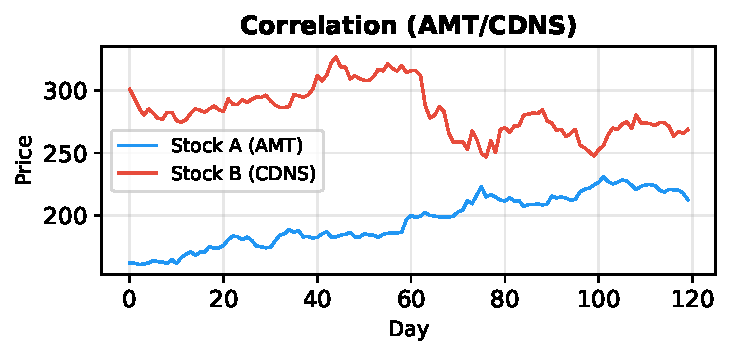
\includegraphics[width=0.95\textwidth]{figures/example_F2_correlation.pdf}
\vspace{4pt}

\textbf{Task: Correlation --- Tickers: AMT vs CDNS --- GT: (B) Negative correlation} \\[4pt]
\begin{minipage}{0.95\textwidth}
\fbox{\parbox{\dimexpr\textwidth-2\fboxsep-2\fboxrule}{
\textbf{Input:} You are analyzing the relationship between two stocks. Stock A (AMT) and Stock B (CDNS) daily closing prices (120 days each): [\textit{prices shown above}]. Determine the correlation between their daily returns. \\
\hspace{6pt}(A) Positive \\
\hspace{6pt}(B) Negative \\
\hspace{6pt}(C) No significant correlation
}} \\[4pt]
\fbox{\parbox{\dimexpr\textwidth-2\fboxsep-2\fboxrule}{
\textbf{Output:} \\[6pt]
\texttt{<think>} \\[4pt]
Step 1 --- Compare price changes in 12 periods ($\sim$10 days each): \\
\hspace{1em}Days 1-10: A=+1.6\%, B=$-$6.0\% \\
\hspace{1em}Days 11-20: A=+7.8\%, B=+3.2\% \\
\hspace{1em}Days 21-30: A=$-$1.0\%, B=+4.5\% \\
\hspace{1em}Days 31-40: A=+2.3\%, B=$-$5.1\% \\
\hspace{1em}Days 41-50: A=$-$0.8\%, B=+1.9\% \\
\hspace{1em}Days 51-60: A=+3.1\%, B=$-$2.4\% \\
\hspace{1em}Days 61-70: A=$-$2.6\%, B=+4.0\% \\
\hspace{1em}Days 71-80: A=+1.5\%, B=$-$1.8\% \\
\hspace{1em}Days 81-90: A=$-$1.9\%, B=+2.7\% \\
\hspace{1em}Days 91-100: A=+0.4\%, B=$-$0.6\% \\
\hspace{1em}Days 101-110: A=$-$1.5\%, B=+2.2\% \\
\hspace{1em}Days 111-120: A=+2.4\%, B=$-$3.1\% \\[6pt]
Step 2 --- Pattern: \\
When A rises, B tends to fall, and when A falls, B tends to rise. The two stocks move in opposite directions across most periods. \\[6pt]
Step 3 --- negative correlation $\rightarrow$ (B). \\[4pt]
\texttt{</think>} \\
\texttt{<answer>(B)</answer>}
}}
\end{minipage}
\caption{(Multi-Assessment) Example of Correlation task.}
\end{figure}

%%% F5 VOLATILITY %%%
\begin{figure}[h]
\centering
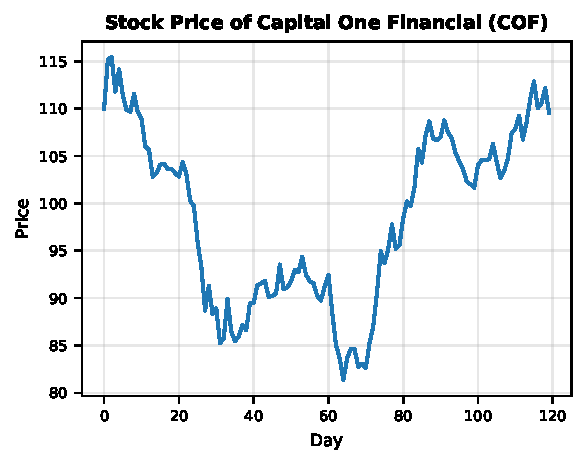
\includegraphics[width=0.95\textwidth]{figures/example_F5_volatility.pdf}
\vspace{4pt}

\textbf{Task: Volatility Regime --- Ticker: COF --- GT: (B) Normal volatility} \\[4pt]
\begin{minipage}{0.95\textwidth}
\fbox{\parbox{\dimexpr\textwidth-2\fboxsep-2\fboxrule}{
\textbf{Input:} You are analyzing the stock COF. Below are the daily closing prices (120 days): [\textit{prices shown above}]. Compute the ratio of recent (last 20 days) to overall (120-day) volatility. \\
\hspace{6pt}(A) Low ($<$0.6) \\
\hspace{6pt}(B) Normal (0.6--1.6) \\
\hspace{6pt}(C) High ($>$1.6)
}} \\[4pt]
\fbox{\parbox{\dimexpr\textwidth-2\fboxsep-2\fboxrule}{
\textbf{Output:} \\[6pt]
\texttt{<think>} \\[4pt]
Step 1 --- Compute daily returns from prices: \\
\hspace{1em}e.g., (54.32$\rightarrow$54.51): +0.35\%, (54.51$\rightarrow$54.10): $-$0.75\%, (54.10$\rightarrow$54.78): +1.26\% \\
\hspace{1em}\ldots \\[6pt]
Step 2 --- Overall volatility (std of all returns): 2.02\% \\[6pt]
Step 3 --- Recent 20-day volatility: 1.50\% \\[6pt]
Step 4 --- Ratio = 1.50 / 2.02 = 0.74 \\
Recent volatility is close to the long-term average --- normal conditions. \\
$\rightarrow$ (B) normal volatility. \\[4pt]
\texttt{</think>} \\
\texttt{<answer>(B)</answer>}
}}
\end{minipage}
\caption{(Single-Assessment) Example of Volatility Regime task.}
\vspace{15pt}
\end{figure}

%%% F6 TREND %%%
\begin{figure}[h]
\centering
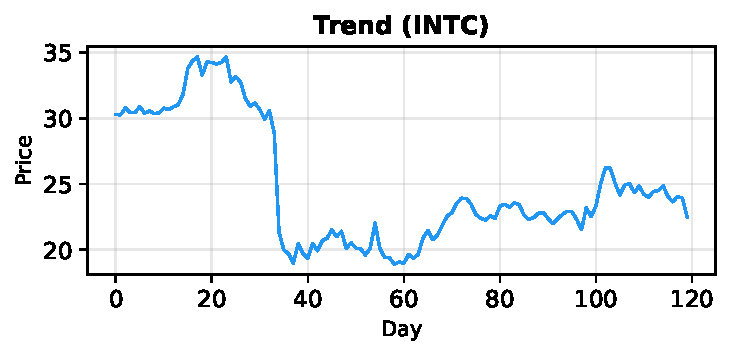
\includegraphics[width=0.95\textwidth]{figures/example_F6_trend.pdf}
\vspace{4pt}

\textbf{Task: Trend Direction --- Ticker: INTC --- GT: (E) Strong Downtrend} \\[4pt]
\begin{minipage}{0.95\textwidth}
\fbox{\parbox{\dimexpr\textwidth-2\fboxsep-2\fboxrule}{
\textbf{Input:} You are analyzing the stock INTC. Below are the daily closing prices (120 days): [\textit{prices shown above}]. Classify the overall trend direction. \\
\hspace{6pt}(A) Strong Uptrend ($>$20\%) \\
\hspace{6pt}(B) Mild Uptrend (5--20\%) \\
\hspace{6pt}(C) Sideways ($-$5\% to +5\%) \\
\hspace{6pt}(D) Mild Downtrend (5--20\% decline) \\
\hspace{6pt}(E) Strong Downtrend ($>$20\% decline)
}} \\[4pt]
\fbox{\parbox{\dimexpr\textwidth-2\fboxsep-2\fboxrule}{
\textbf{Output:} \\[6pt]
\texttt{<think>} \\[4pt]
Step 1 --- Read start and end prices: \\
Start (day 1): 30.27 \\
End (day 120): 22.47 \\[6pt]
Step 2 --- Compute cumulative return: \\
Return = (22.47 $-$ 30.27) / 30.27 = $-$25.8\% \\[6pt]
Step 3 --- Classify: \\
$-$25.8\% $\rightarrow$ (E) Strong Downtrend ($<-$20\%). \\[4pt]
\texttt{</think>} \\
\texttt{<answer>(E)</answer>}
}}
\end{minipage}
\caption{(Single-Assessment) Example of Trend Direction task.}
\end{figure}

\clearpage
\subsection{Prediction Tasks (Scenario-Aware CoT)}

%%% F3 EVENT %%%
\begin{figure}[h]
\vspace{-10pt}
\centering
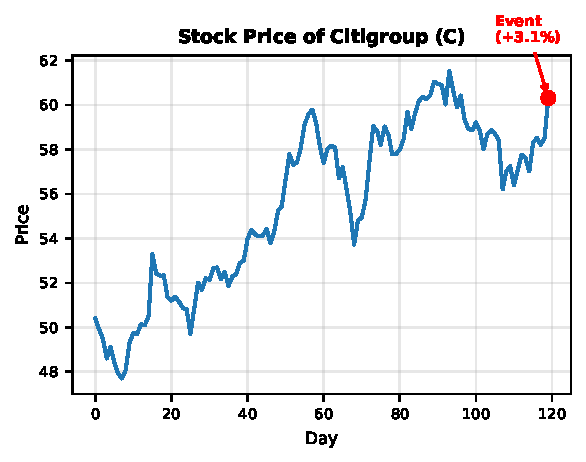
\includegraphics[width=0.73\textwidth]{figures/example_F3_event.pdf}
\vspace{1pt}

\textbf{Task: Event Response --- Ticker: C --- GT: (B) Persistence} \\[4pt]
\begin{minipage}{0.95\textwidth}
\fbox{\parbox{\dimexpr\textwidth-2\fboxsep-2\fboxrule}{
\textbf{Input:} You are analyzing the stock C. Below are the daily closing prices (120 days): [\textit{prices shown above}]. The stock just experienced a significant positive shock. Predict the outcome over the next 10 days. \\
\hspace{6pt}(A) Mean-reversion \\
\hspace{6pt}(B) Persistence
}} \\[4pt]
\fbox{\parbox{\dimexpr\textwidth-2\fboxsep-2\fboxrule}{
\textbf{Output:} \\[6pt]
\texttt{<think>} \\[4pt]
Step 1 --- Event: positive shock, z=2.20, return=+1.85\%. \\[6pt]
Step 2 --- Pre-event trend: flat. \\[6pt]
Step 3 --- Scenario analysis: \\
\hspace{2em}$\bullet$ \textit{Base case} (most probable --- no major external events): \\
\hspace{2.7em}The positive shock reflects genuine new information being priced in. The market continues to absorb the news over the following days, sustaining the move in the same direction. \\[4pt]
\hspace{2em}$\bullet$ \textit{Adverse scenario} (external shock reverses expectation): \\
\hspace{2.7em}Mean-reversion forces kick in as profit-taking and overreaction corrections pull the price back toward pre-event levels. \\[4pt]
\hspace{2em}$\bullet$ \textit{Favorable scenario} (catalyst strengthens expectation): \\
\hspace{2.7em}Additional confirming news (e.g., earnings beat, upgrade) amplifies the move and accelerates persistence. \\[6pt]
Step 4 --- Scenario assessment: \\
The base case and favorable scenario (2 of 3) support Persistence. \\
The adverse scenario requires a specific external trigger not present in current data. \\
Without new information, the base case is the most probable outcome. \\[6pt]
Step 5 --- Judgment: Base case favors Persistence $\rightarrow$ (B). \\[4pt]
\texttt{</think>} \\
\texttt{<answer>(B)</answer>}
}}
\end{minipage}
\caption{(Single-Prediction) Example of Event Response task.}
\vspace{-40pt}
\end{figure}

%%% F7 S/R %%%
\begin{figure}[h]
\centering
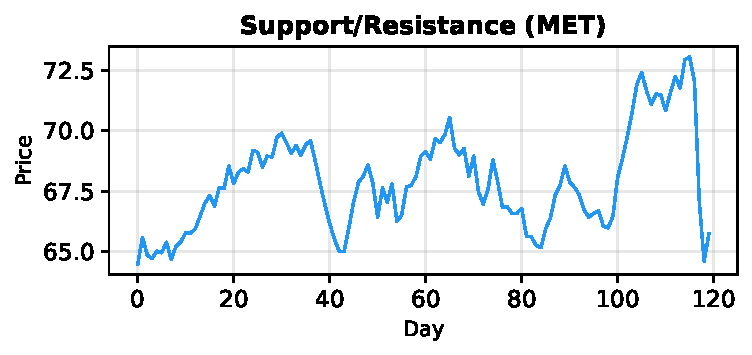
\includegraphics[width=0.95\textwidth]{figures/example_F7_breakout.pdf}
\vspace{4pt}

\textbf{Task: Support/Resistance --- Ticker: MET --- GT: (B) Bounce} \\[4pt]
\begin{minipage}{0.95\textwidth}
\fbox{\parbox{\dimexpr\textwidth-2\fboxsep-2\fboxrule}{
\textbf{Input:} You are analyzing the stock MET. Below are the daily closing prices (120 days): [\textit{prices shown above}]. The stock is currently near a key support level. Predict the behavior over the next 10 days. \\
\hspace{6pt}(A) Breakout \\
\hspace{6pt}(B) Bounce
}} \\[4pt]
\fbox{\parbox{\dimexpr\textwidth-2\fboxsep-2\fboxrule}{
\textbf{Output:} \\[6pt]
\texttt{<think>} \\[4pt]
Step 1 --- Key level: support at 64.47. \\[6pt]
Step 2 --- Proximity: 1.9\%. \\[6pt]
Step 3 --- Scenario analysis: \\
\hspace{2em}$\bullet$ \textit{Base case} (most probable --- no major external events): \\
\hspace{2.7em}The key level holds as institutional orders defend it. Price reverses direction after testing the level. \\[4pt]
\hspace{2em}$\bullet$ \textit{Adverse scenario} (external shock reverses expectation): \\
\hspace{2.7em}Sustained pressure eventually overwhelms the level, leading to a delayed breakout. \\[4pt]
\hspace{2em}$\bullet$ \textit{Favorable scenario} (catalyst strengthens expectation): \\
\hspace{2.7em}A strong bounce off the level triggers a significant reversal move in the opposite direction. \\[6pt]
Step 4 --- Scenario assessment: \\
The base case and favorable scenario (2 of 3) support Bounce. \\
The adverse scenario requires a specific external trigger not present in current data. \\
Without new information, the base case is the most probable outcome. \\[6pt]
Step 5 --- Judgment: Base case favors Bounce $\rightarrow$ (B). \\[4pt]
\texttt{</think>} \\
\texttt{<answer>(B)</answer>}
}}
\end{minipage}
\caption{(Single-Prediction) Example of Support/Resistance task.}
\end{figure}

%%% F4 MOMENTUM %%%
\begin{figure}[h]
\centering
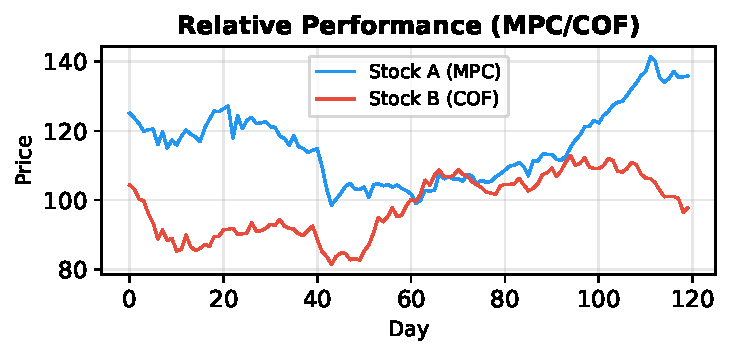
\includegraphics[width=0.95\textwidth]{figures/example_F4_momentum.pdf}
\vspace{4pt}

\textbf{Task: Relative Performance --- Tickers: MPC vs COF --- GT: (A) Stock A outperforms} \\[4pt]
\begin{minipage}{0.95\textwidth}
\fbox{\parbox{\dimexpr\textwidth-2\fboxsep-2\fboxrule}{
\textbf{Input:} You are comparing two stocks. Stock A (MPC) and Stock B (COF) daily closing prices (120 days each): [\textit{prices shown above}]. Predict which stock will have a higher return over the next 20 days. \\
\hspace{6pt}(A) Stock A outperforms \\
\hspace{6pt}(B) Stock B outperforms
}} \\[4pt]
\fbox{\parbox{\dimexpr\textwidth-2\fboxsep-2\fboxrule}{
\textbf{Output:} \\[6pt]
\texttt{<think>} \\[4pt]
Step 1 --- Comparing MPC vs COF. \\[6pt]
Step 2 --- Forward window: 20 days. \\[6pt]
Step 3 --- Scenario analysis: \\
\hspace{2em}$\bullet$ \textit{Base case} (most probable --- no major external events): \\
\hspace{2.7em}Stock A's recent strengthening continues, while Stock B's momentum fades. The relative performance gap widens further in A's favor. \\[4pt]
\hspace{2em}$\bullet$ \textit{Adverse scenario} (external shock reverses expectation): \\
\hspace{2.7em}A company-specific headwind hits Stock A (e.g., earnings miss, regulatory issue), eroding its lead. \\[4pt]
\hspace{2em}$\bullet$ \textit{Favorable scenario} (catalyst strengthens expectation): \\
\hspace{2.7em}Sector tailwinds (e.g., favorable commodity prices) boost Stock A and widen its outperformance. \\[6pt]
Step 4 --- Scenario assessment: \\
The base case and favorable scenario (2 of 3) support Stock A outperforms. \\
The adverse scenario requires a specific external trigger not present in current data. \\
Without new information, the base case is the most probable outcome. \\[6pt]
Step 5 --- Judgment: Base case favors Stock A outperforms $\rightarrow$ (A). \\[4pt]
\texttt{</think>} \\
\texttt{<answer>(A)</answer>}
}}
\end{minipage}
\caption{(Multi-Prediction) Example of Relative Performance task.}
\vspace{15pt}
\end{figure}

%%% F8 DD RECOVERY %%%
\begin{figure}[h]
\centering
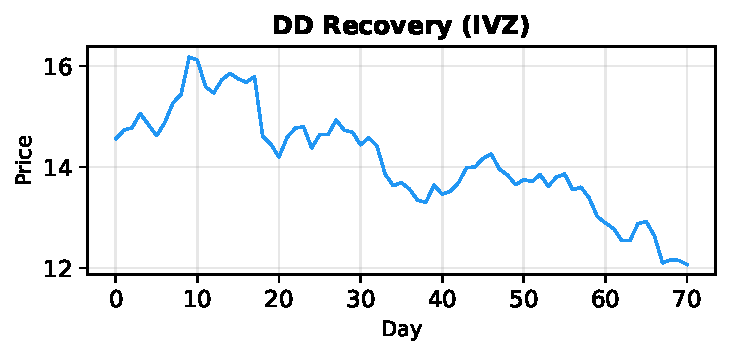
\includegraphics[width=0.95\textwidth]{figures/example_F8_drawdown_recovery.pdf}
\vspace{4pt}

\textbf{Task: Drawdown Recovery --- Ticker: IVZ --- GT: (B) Deepens} \\[4pt]
\begin{minipage}{0.95\textwidth}
\fbox{\parbox{\dimexpr\textwidth-2\fboxsep-2\fboxrule}{
\textbf{Input:} You are analyzing the stock IVZ. Below are the daily closing prices: [\textit{prices shown above}]. The stock has experienced a drawdown of 25.4\% from its recent peak. Predict the behavior over the next 20 days. \\
\hspace{6pt}(A) Recovery \\
\hspace{6pt}(B) Deepens
}} \\[4pt]
\fbox{\parbox{\dimexpr\textwidth-2\fboxsep-2\fboxrule}{
\textbf{Output:} \\[6pt]
\texttt{<think>} \\[4pt]
Step 1 --- Drawdown: 25.4\% (peak=16.18, current=12.07). \\[6pt]
Step 2 --- Peak was 62 days ago. \\[6pt]
Step 3 --- Scenario analysis: \\
\hspace{2em}$\bullet$ \textit{Base case} (most probable --- no major external events): \\
\hspace{2.7em}Selling pressure continues as the fundamental weakness persists. The drawdown deepens before eventually finding a floor. \\[4pt]
\hspace{2em}$\bullet$ \textit{Adverse scenario} (external shock reverses expectation): \\
\hspace{2.7em}A surprise positive development reverses the decline --- but this requires a specific external trigger. \\[4pt]
\hspace{2em}$\bullet$ \textit{Favorable scenario} (catalyst strengthens expectation): \\
\hspace{2.7em}The decline accelerates as market-wide risk-off sentiment compounds the stock-specific weakness. \\[6pt]
Step 4 --- Scenario assessment: \\
The base case and favorable scenario (2 of 3) support Deepens. \\
The adverse scenario requires a specific external trigger not present in current data. \\
Without new information, the base case is the most probable outcome. \\[6pt]
Step 5 --- Judgment: Base case favors Deepens $\rightarrow$ (B). \\[4pt]
\texttt{</think>} \\
\texttt{<answer>(B)</answer>}
}}
\end{minipage}
\caption{(Single-Prediction) Example of Drawdown Recovery task.}
\end{figure}

%%% F9 VOL FORECAST %%%
\begin{figure}[h]
\centering
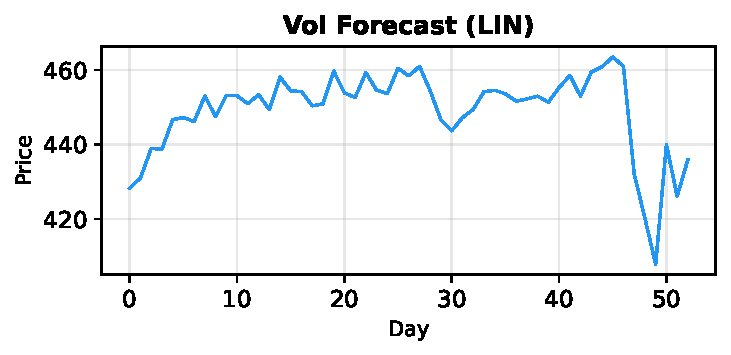
\includegraphics[width=0.95\textwidth]{figures/example_F9_volatility_forecast.pdf}
\vspace{4pt}

\textbf{Task: Volatility Forecast --- Ticker: LIN --- GT: (B) Volatility decreases} \\[4pt]
\begin{minipage}{0.95\textwidth}
\fbox{\parbox{\dimexpr\textwidth-2\fboxsep-2\fboxrule}{
\textbf{Input:} You are analyzing the stock LIN. Below are the daily closing prices: [\textit{prices shown above}]. The current volatility ratio (recent 20-day vs overall) is 1.43. Predict how volatility will change over the next 20 days. \\
\hspace{6pt}(A) Increases \\
\hspace{6pt}(B) Decreases
}} \\[4pt]
\fbox{\parbox{\dimexpr\textwidth-2\fboxsep-2\fboxrule}{
\textbf{Output:} \\[6pt]
\texttt{<think>} \\[4pt]
Step 1 --- Vol: recent=2.59\%, long=1.81\%, ratio=1.43. \\[6pt]
Step 2 --- Volatility pattern assessed. \\[6pt]
Step 3 --- Scenario analysis: \\
\hspace{2em}$\bullet$ \textit{Base case} (most probable --- no major external events): \\
\hspace{2.7em}Volatility mean-reverts toward the long-run level as the recent shock dissipates and the market normalizes. \\[4pt]
\hspace{2em}$\bullet$ \textit{Adverse scenario} (external shock reverses expectation): \\
\hspace{2.7em}A new source of uncertainty (earnings, macro news) triggers another volatility spike. \\[4pt]
\hspace{2em}$\bullet$ \textit{Favorable scenario} (catalyst strengthens expectation): \\
\hspace{2.7em}Market calming accelerates as uncertainty resolves, pushing volatility down faster than baseline. \\[6pt]
Step 4 --- Scenario assessment: \\
The base case and favorable scenario (2 of 3) support Vol decreases. \\
The adverse scenario requires a specific external trigger not present in current data. \\
Without new information, the base case is the most probable outcome. \\[6pt]
Step 5 --- Judgment: Base case favors Vol decreases $\rightarrow$ (B). \\[4pt]
\texttt{</think>} \\
\texttt{<answer>(B)</answer>}
}}
\end{minipage}
\caption{(Single-Prediction) Example of Volatility Forecast task.}
\vspace{15pt}
\end{figure}

%%% F10 PAIR CONVERGENCE %%%
\begin{figure}[h]
\centering
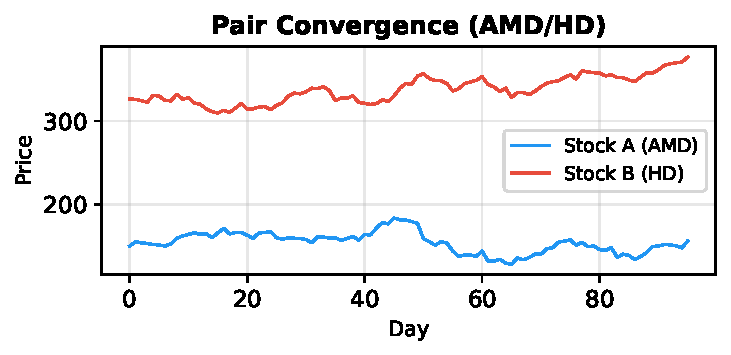
\includegraphics[width=0.95\textwidth]{figures/example_F10_pair_convergence.pdf}
\vspace{4pt}

\textbf{Task: Pair Convergence --- Tickers: AMD vs HD --- GT: (B) Divergence} \\[4pt]
\begin{minipage}{0.95\textwidth}
\fbox{\parbox{\dimexpr\textwidth-2\fboxsep-2\fboxrule}{
\textbf{Input:} You are comparing two stocks. Stock A (AMD) and Stock B (HD) daily closing prices: [\textit{prices shown above}]. The price spread (normalized difference) is 0.113. Predict how the spread will change over the next 20 days. \\
\hspace{6pt}(A) Convergence \\
\hspace{6pt}(B) Divergence
}} \\[4pt]
\fbox{\parbox{\dimexpr\textwidth-2\fboxsep-2\fboxrule}{
\textbf{Output:} \\[6pt]
\texttt{<think>} \\[4pt]
Step 1 --- Pair: AMD, HD. \\[6pt]
Step 2 --- Current spread: 0.113. \\[6pt]
Step 3 --- Scenario analysis: \\
\hspace{2em}$\bullet$ \textit{Base case} (most probable --- no major external events): \\
\hspace{2.7em}Different fundamentals sustain the widening spread. The divergence continues as the two stocks respond to distinct sector dynamics. \\[4pt]
\hspace{2em}$\bullet$ \textit{Adverse scenario} (external shock reverses expectation): \\
\hspace{2.7em}A common catalyst (e.g., index rebalancing, macro shock) narrows the spread by forcing temporary co-movement. \\[4pt]
\hspace{2em}$\bullet$ \textit{Favorable scenario} (catalyst strengthens expectation): \\
\hspace{2.7em}Company-specific events accelerate the divergence further as one stock's fundamentals diverge from the other's. \\[6pt]
Step 4 --- Scenario assessment: \\
The base case and favorable scenario (2 of 3) support Divergence. \\
The adverse scenario requires a specific external trigger not present in current data. \\
Without new information, the base case is the most probable outcome. \\[6pt]
Step 5 --- Judgment: Base case favors Divergence $\rightarrow$ (B). \\[4pt]
\texttt{</think>} \\
\texttt{<answer>(B)</answer>}
}}
\end{minipage}
\caption{(Multi-Prediction) Example of Pair Convergence task.}
\end{figure}




% \clearpage
% \section{Prediction Calibration}
% \label{app:calibration}
%
% The Brier score~\cite{brier1950} is a proper scoring rule that measures the accuracy of probabilistic predictions.
% For a binary classification task, it is defined as:
% \[
% \text{BS} = \frac{1}{N} \sum_{i=1}^{N} (f_i - o_i)^2
% \]
% where $f_i \in [0, 1]$ is the predicted probability and $o_i \in \{0, 1\}$ is the actual outcome.
% Lower Brier scores indicate better calibration, with 0 representing perfect prediction and 0.25 corresponding to random guessing on a balanced binary task.
% Since our framework outputs hard classification labels rather than soft probabilities, we set $f_i = 1$ when the model predicts the correct class and $f_i = 0$ otherwise, reducing the Brier score to $(1 - \text{accuracy})$.
%
% Table~\ref{tab:brier} reports per-task Brier scores on the six binary prediction tasks for FinSTaR and two zero-shot baselines.
% FinSTaR achieves the best Brier score on all six tasks, with the largest improvements on Support/Resistance and Volatility Forecast.
% Extending to soft probabilistic outputs (e.g., via confidence calibration) is a promising direction for future work.
%
% \begin{table}[h]
% \centering
% \caption{\textbf{Brier scores on prediction tasks (Test A).} Lower is better. FinSTaR achieves the best score on all six tasks.}
% \label{tab:brier}
% \vspace{5pt}
% \adjustbox{max width=\textwidth}{
% \begin{tabular}{l|cc|cc|cc}
% \toprule
%  & \multicolumn{2}{c|}{\textbf{Qwen2.5-7B (ZS)}} & \multicolumn{2}{c|}{\textbf{TimeOmni-1 (ZS)}} & \multicolumn{2}{c}{\textbf{FinSTaR (Ours)}} \\
% \cmidrule(lr){2-3} \cmidrule(lr){4-5} \cmidrule(lr){6-7}
% \textbf{Task} & \textbf{Acc.} & \textbf{Brier} & \textbf{Acc.} & \textbf{Brier} & \textbf{Acc.} & \textbf{Brier} \\
% \midrule
% Event Response & 52.2 & 0.478 & 49.1 & 0.509 & \textbf{57.2} & \textbf{0.428} \\
% Support/Resistance & 51.2 & 0.488 & 54.1 & 0.459 & \textbf{80.5} & \textbf{0.195} \\
% Relative Performance & 49.2 & 0.508 & 50.7 & 0.493 & \textbf{51.5} & \textbf{0.485} \\
% Drawdown Recovery & 54.1 & 0.459 & 59.3 & 0.407 & \textbf{74.4} & \textbf{0.256} \\
% Volatility Forecast & 44.9 & 0.551 & 58.2 & 0.418 & \textbf{79.5} & \textbf{0.205} \\
% Pair Convergence & 50.4 & 0.496 & 48.4 & 0.516 & \textbf{65.8} & \textbf{0.342} \\
% \midrule
% Average & 50.3 & 0.497 & 53.3 & 0.467 & \textbf{68.2} & \textbf{0.319} \\
% \bottomrule
% \end{tabular}
% }
% \end{table}

% \begin{figure}[h]
% \centering
% \begin{subfigure}[t]{0.48\textwidth}
% \includegraphics[width=\textwidth]{figures/placeholder_epoch_assess.pdf}
% \caption{Assessment tasks converge by EP1--2.}
% \end{subfigure}
% \hfill
% \begin{subfigure}[t]{0.48\textwidth}
% \includegraphics[width=\textwidth]{figures/placeholder_epoch_predict.pdf}
% \caption{Prediction tasks improve until EP3--4.}
% \end{subfigure}
% \caption{\textbf{Epoch progression.} Assessment tasks saturate early, while prediction tasks require more training to internalize scenario reasoning.}
% \label{fig:epoch}
% \end{figure}

% Data Efficiency table moved to main text (Section 6)

\clearpage
\section{Comparison with Other Methods}
\label{app:qualitative}

We present three qualitative examples per task where only FinSTaR answers correctly while both baselines (Qwen2.5-7B and TimeOmni-1-7B, zero-shot) fail.

% \clearpage
\subsection{Drawdown (Assessment)}


\noindent
\textbf{Example 1: Drawdown (Assessment) --- Ticker: ABBV --- GT: (C)}
\vspace{2pt}

\noindent
\begin{minipage}[t]{0.28\textwidth}
\colorbox{red!8}{\parbox{\dimexpr\textwidth-2\fboxsep}{
\textbf{Qwen2.5-7B} \textcolor{red}{(B)} \ding{55}\\[2pt]
\tiny
[think]\newline To determine the current drawdown phase of ABBV, we need to identify the recent peak price and then calculate how far the current price is from that peak.\newline 1. Identify the highest price in the given data.\newline 2. Calculate the difference between the highest price and the current price.\newline 3. Determine the percentage decline based on the highest price.\newline From the data provided, the highest price is 17 [...]
}}
\end{minipage}
\hfill
\begin{minipage}[t]{0.28\textwidth}
\colorbox{red!8}{\parbox{\dimexpr\textwidth-2\fboxsep}{
\textbf{TimeOmni-1} \textcolor{red}{(B)} \ding{55}\\[2pt]
\tiny
[think]\newline Step 1: Identify the recent peak  \newline - The data covers 120 trading days.  \newline - The highest value in the series is 170.00 (last value), which is at index 119.  \newline - The previous day's price is 168.75 (index 118).  \newline - The day before that is 168.68 (index 117).  \newline - The day before that is 165.54 (index 116).  \newline - The day before that is 156.74 (index 115).  \newline - The day before that is 158.70 (index 114) [...]
}}
\end{minipage}
\hfill
\begin{minipage}[t]{0.41\textwidth}
\colorbox{green!10}{\parbox{\dimexpr\textwidth-2\fboxsep}{
\textbf{FinSTaR (Ours)} \textcolor{green!50!black}{(C)} \ding{51}\\[2pt]
\tiny
[think]\newline Step 1 -- Find the peak price:\newline Scanning the 120-day series, the highest price is 170.00 (around day 108).\newline Step 2 -- Current price:\newline The last price in the series is 152.33.\newline Step 3 -- Calculate drawdown:\newline Drawdown = (Peak - Current) / Peak = (170.00 - 152.33) / 170.00 = 10.4 pct\newline Step 4 -- Classify:\newline 10.4 pct is between 10 pct and 20 pct, which corresponds to (C) Correction.\newline [/think]\newline [answer]C[/answer]
}}
\end{minipage}
\vspace{8pt}


\noindent
\textbf{Example 2: Drawdown (Assessment) --- Ticker: DHR --- GT: (C)}
\vspace{2pt}

\noindent
\begin{minipage}[t]{0.28\textwidth}
\colorbox{red!8}{\parbox{\dimexpr\textwidth-2\fboxsep}{
\textbf{Qwen2.5-7B} \textcolor{red}{(A)} \ding{55}\\[2pt]
\tiny
[think]\newline To determine the current drawdown phase of the stock DHR, we need to identify its recent peak price and then compare the current price to this peak.\newline 1. Identify the Recent Peak Price:\newline    - The data provided shows the most recent 120 trading days' closing prices.\newline    - The highest value in this list is 211.53, which occurred on the last day of the provided data.\newline 2. Determine the Curren [...]
}}
\end{minipage}
\hfill
\begin{minipage}[t]{0.28\textwidth}
\colorbox{red!8}{\parbox{\dimexpr\textwidth-2\fboxsep}{
\textbf{TimeOmni-1} \textcolor{red}{(A)} \ding{55}\\[2pt]
\tiny
[think]\newline Step 1: Identify the most recent peak  \newline - The data shows a clear upward trend with some fluctuations, but the highest value in the series is at the end: 211.53 (last value).\newline - The previous high before this was 211.47 (second-to-last value), so the most recent peak is at or very close to the last value.\newline Step 2: Estimate the current price  \newline - The most recent value is 211.53.\newline - The next-to-la [...]
}}
\end{minipage}
\hfill
\begin{minipage}[t]{0.41\textwidth}
\colorbox{green!10}{\parbox{\dimexpr\textwidth-2\fboxsep}{
\textbf{FinSTaR (Ours)} \textcolor{green!50!black}{(C)} \ding{51}\\[2pt]
\tiny
[think]\newline Step 1 -- Find the peak price:\newline Scanning the 120-day series, the highest price is 211.53 (around day 103).\newline Step 2 -- Current price:\newline The last price in the series is 189.45.\newline Step 3 -- Calculate drawdown:\newline Drawdown = (Peak - Current) / Peak = (211.53 - 189.45) / 211.53 = 10.5 pct\newline Step 4 -- Classify:\newline 10.5 pct is between 10 pct and 20 pct, which corresponds to (C) Correction.\newline [/think]\newline [answer]C[/answer]
}}
\end{minipage}
\vspace{8pt}


\noindent
\textbf{Example 3: Drawdown (Assessment) --- Ticker: CRWD --- GT: (C)}
\vspace{2pt}

\noindent
\begin{minipage}[t]{0.28\textwidth}
\colorbox{red!8}{\parbox{\dimexpr\textwidth-2\fboxsep}{
\textbf{Qwen2.5-7B} \textcolor{red}{(B)} \ding{55}\\[2pt]
\tiny
[think]\newline To determine the current drawdown phase of the stock CRWD, we need to identify the recent peak price and then compare the current price to this peak.\newline 1. Identify the Recent Peak Price:\newline    - The data provided shows the most recent 120 trading days' closing prices.\newline    - The highest value in the list is 334.55, which occurred on one of the last few days.\newline 2. Determine the Current Price:* [...]
}}
\end{minipage}
\hfill
\begin{minipage}[t]{0.28\textwidth}
\colorbox{red!8}{\parbox{\dimexpr\textwidth-2\fboxsep}{
\textbf{TimeOmni-1} \textcolor{red}{(B)} \ding{55}\\[2pt]
\tiny
[think]\newline Step 1: Identify the recent peak  \newline - The data shows a clear upward trend with a few dips and rises.  \newline - The highest value in the series is 334.55 (at index 95).  \newline - The last value is 310.77 (index 119), which is lower than the peak but still relatively high.\newline Step 2: Estimate the current price  \newline - The last value is 310.77.  \newline - The previous value was 329.57 (index 118), so there has been a d [...]
}}
\end{minipage}
\hfill
\begin{minipage}[t]{0.41\textwidth}
\colorbox{green!10}{\parbox{\dimexpr\textwidth-2\fboxsep}{
\textbf{FinSTaR (Ours)} \textcolor{green!50!black}{(C)} \ding{51}\\[2pt]
\tiny
[think]\newline Step 1 -- Find the peak price:\newline Scanning the 120-day series, the highest price is 334.55 (around day 76).\newline Step 2 -- Current price:\newline The last price in the series is 299.15.\newline Step 3 -- Calculate drawdown:\newline Drawdown = (Peak - Current) / Peak = (334.55 - 299.15) / 334.55 = 10.6 pct\newline Step 4 -- Classify:\newline 10.6 pct is between 10 pct and 20 pct, which corresponds to (C) Correction.\newline [/think]\newline [answer]C[/answer]
}}
\vspace{-30pt}
\end{minipage}

\clearpage
\subsection{Correlation (Assessment)}


\noindent
\textbf{Example 1: Correlation (Assessment) --- Ticker: AMD\_BAC --- GT: (A)}
\vspace{2pt}

\noindent
\begin{minipage}[t]{0.28\textwidth}
\colorbox{red!8}{\parbox{\dimexpr\textwidth-2\fboxsep}{
\textbf{Qwen2.5-7B} \textcolor{red}{(C)} \ding{55}\\[2pt]
\tiny
[think]To determine the correlation between the daily returns of Stock A and Stock B, we need to calculate the correlation coefficient. However, given the complexity and the fact that we are asked to choose from predefined options, we can analyze the general trend visually or through a simplified approach.\newline Firstly, let's observe the trends:\newline - Stock A's prices show a significant fluctuation with so [...]
}}
\end{minipage}
\hfill
\begin{minipage}[t]{0.28\textwidth}
\colorbox{red!8}{\parbox{\dimexpr\textwidth-2\fboxsep}{
\textbf{TimeOmni-1} \textcolor{red}{(B)} \ding{55}\\[2pt]
\tiny
[think]\newline Step 1: Trend Consistency (Perceptual Matching)\newline - Both Stock A (AMD) and Stock B (BAC) start with relatively stable/flat periods at the beginning.\newline - Both show a gradual rise in the first half of the series (e.g., both increase from  137-144 for AMD and  44-46 for BAC).\newline - Both then experience a decline or stabilization period (e.g., AMD falls from  144 down to  110, BAC falls from  46 down  [...]
}}
\end{minipage}
\hfill
\begin{minipage}[t]{0.41\textwidth}
\colorbox{green!10}{\parbox{\dimexpr\textwidth-2\fboxsep}{
\textbf{FinSTaR (Ours)} \textcolor{green!50!black}{(A)} \ding{51}\\[2pt]
\tiny
[think]\newline Step 1 -- Compare price changes in 12 periods ( 10 days each):\newline   Days 1-10: A=+2.8 pct, B=+1.2 pct\newline   Days 11-20: A=-14.3 pct, B=-7.2 pct\newline   Days 21-30: A=+8.6 pct, B=+2.8 pct\newline   Days 31-40: A=-2.8 pct, B=-0.6 pct\newline   Days 41-50: A=-8.9 pct, B=+1.5 pct\newline   Days 51-60: A=+3.6 pct, B=-5.1 pct\newline   Days 61-70: A=-10.8 pct, B=-7.5 pct\newline   Days 71-80: A=+10.0 pct, B=+2.6 pct\newline   Days 81-90: A=-23.9 pct, B=-12.4 pct\newline   Days 91-100: A=+3.1 pct, B=+8.8 pct\newline   Days 101-110: A=+10.1 pct, B=+11.2 pct\newline   Days 111-120: A=+20.0 pct, B=+8.7 pct\newline Step 2 -- Pattern:\newline When A rises, B also tends to rise, and when A falls, B also falls. The magnitudes are similar.\newline Step 3 -- positive correlation -> (A).\newline [/think]\newline [answer]A[/answer]
}}
\end{minipage}
\vspace{8pt}


\noindent
\textbf{Example 2: Correlation (Assessment) --- Ticker: CRM\_DECK --- GT: (A)}
\vspace{2pt}

\noindent
\begin{minipage}[t]{0.28\textwidth}
\colorbox{red!8}{\parbox{\dimexpr\textwidth-2\fboxsep}{
\textbf{Qwen2.5-7B} \textcolor{red}{(B)} \ding{55}\\[2pt]
\tiny
[think]To determine the correlation between the daily returns of Stock A and Stock B, we need to calculate the correlation coefficient. However, given the complexity and the fact that we are only asked to determine the nature of the correlation (positive, negative, or no significant), we can infer this by observing the general trend of the price movements.\newline For Stock A (CRM):\newline - The prices show some [...]
}}
\end{minipage}
\hfill
\begin{minipage}[t]{0.28\textwidth}
\colorbox{red!8}{\parbox{\dimexpr\textwidth-2\fboxsep}{
\textbf{TimeOmni-1} \textcolor{red}{(B)} \ding{55}\\[2pt]
\tiny
[think]\newline Step 1: Trend Consistency (Perceptual Matching)\newline - Both Stock A (CRM) and Stock B (DECK) start with relatively stable values for the first few days.\newline - Around day 10-15, both begin to rise: CRM goes from  282 to  339, DECK from  152 to  178.\newline - Both peak around day 15-16, then both decline slightly.\newline - Both show a pronounced rise again starting around day 25-30: CRM rises from  320 to  365, DE [...]
}}
\end{minipage}
\hfill
\begin{minipage}[t]{0.41\textwidth}
\colorbox{green!10}{\parbox{\dimexpr\textwidth-2\fboxsep}{
\textbf{FinSTaR (Ours)} \textcolor{green!50!black}{(A)} \ding{51}\\[2pt]
\tiny
[think]\newline Step 1 -- Compare price changes in 12 periods ( 10 days each):\newline   Days 1-10: A=+3.4 pct, B=+5.3 pct\newline   Days 11-20: A=+8.3 pct, B=+7.8 pct\newline   Days 21-30: A=+2.5 pct, B=+15.1 pct\newline   Days 31-40: A=-4.6 pct, B=+3.0 pct\newline   Days 41-50: A=-2.0 pct, B=+1.5 pct\newline   Days 51-60: A=-2.5 pct, B=+1.3 pct\newline   Days 61-70: A=+3.8 pct, B=-20.3 pct\newline   Days 71-80: A=-4.4 pct, B=-8.1 pct\newline   Days 81-90: A=-11.5 pct, B=-12.3 pct\newline   Days 91-100: A=-4.5 pct, B=-15.3 pct\newline   Days 101-110: A=-3.3 pct, B=-4.8 pct\newline   Days 111-120: A=-6.0 pct, B=-11.8 pct\newline Step 2 -- Pattern:\newline When A rises, B also tends to rise, and when A falls, B also falls. The magnitudes are similar.\newline Step 3 -- positive correlation -> (A).\newline [/think]\newline [answer]A[/answer]
}}
\end{minipage}
\vspace{8pt}


\noindent
\textbf{Example 3: Correlation (Assessment) --- Ticker: MRK\_EL --- GT: (A)}
\vspace{2pt}

\noindent
\begin{minipage}[t]{0.28\textwidth}
\colorbox{red!8}{\parbox{\dimexpr\textwidth-2\fboxsep}{
\textbf{Qwen2.5-7B} \textcolor{red}{(B)} \ding{55}\\[2pt]
\tiny
[think]To determine the correlation between the daily returns of Stock A and Stock B, we need to calculate the correlation coefficient. However, given the complexity and the fact that we are asked to choose from predefined options, we can analyze the general trend visually or through a simplified approach.\newline Firstly, let's observe the trends:\newline - Stock A's prices show fluctuations but generally seem t [...]
}}
\end{minipage}
\hfill
\begin{minipage}[t]{0.28\textwidth}
\colorbox{red!8}{\parbox{\dimexpr\textwidth-2\fboxsep}{
\textbf{TimeOmni-1} \textcolor{red}{(B)} \ding{55}\\[2pt]
\tiny
[think]\newline Step 1: Trend Consistency (Perceptual Matching)\newline - Both Stock A and Stock B start with relatively stable values for about the first 10-15 days.\newline - Around day 15-20, both begin to rise: Stock A goes from  91 to  97, while Stock B rises from  62 to  72.\newline - Both then continue rising, peaking around day 25-30 (A:  98, B:  78).\newline - After this peak, both decline: Stock A falls from  98 down to  85 by [...]
}}
\end{minipage}
\hfill
\begin{minipage}[t]{0.41\textwidth}
\colorbox{green!10}{\parbox{\dimexpr\textwidth-2\fboxsep}{
\textbf{FinSTaR (Ours)} \textcolor{green!50!black}{(A)} \ding{51}\\[2pt]
\tiny
[think]\newline Step 1 -- Compare price changes in 12 periods ( 10 days each):\newline   Days 1-10: A=-2.7 pct, B=-24.0 pct\newline   Days 11-20: A=-3.0 pct, B=+4.6 pct\newline   Days 21-30: A=+4.0 pct, B=+14.0 pct\newline   Days 31-40: A=-4.8 pct, B=-9.0 pct\newline   Days 41-50: A=+1.6 pct, B=-0.8 pct\newline   Days 51-60: A=-3.2 pct, B=+8.8 pct\newline   Days 61-70: A=-7.8 pct, B=-22.2 pct\newline   Days 71-80: A=+2.5 pct, B=+10.4 pct\newline   Days 81-90: A=+3.7 pct, B=-1.9 pct\newline   Days 91-100: A=-1.4 pct, B=-7.1 pct\newline   Days 101-110: A=-11.8 pct, B=-21.5 pct\newline   Days 111-120: A=-4.1 pct, B=+2.7 pct\newline Step 2 -- Pattern:\newline When A rises, B also tends to rise, and when A falls, B also falls. The magnitudes are similar.\newline Step 3 -- positive correlation -> (A).\newline [/think]\newline [answer]A[/answer]
}}
\vspace{-30pt}
\end{minipage}

\clearpage
\subsection{Volatility Regime (Assessment)}


\noindent
\textbf{Example 1: Volatility Regime (Assessment) --- Ticker: BKNG --- GT: (C)}
\vspace{2pt}

\noindent
\begin{minipage}[t]{0.28\textwidth}
\colorbox{red!8}{\parbox{\dimexpr\textwidth-2\fboxsep}{
\textbf{Qwen2.5-7B} \textcolor{red}{(B)} \ding{55}\\[2pt]
\tiny
[think]\newline To determine the volatility regimes, we need to calculate both the recent (last 20 days) and overall (120-day) volatility. Volatility can be measured using the standard deviation of the returns.\newline 1. Calculate the daily returns for each day.\newline 2. Compute the standard deviation of these returns for the last 20 days (recent volatility).\newline 3. Compute the standard deviation of these returns for the  [...]
}}
\end{minipage}
\hfill
\begin{minipage}[t]{0.28\textwidth}
\colorbox{red!8}{\parbox{\dimexpr\textwidth-2\fboxsep}{
\textbf{TimeOmni-1} \textcolor{red}{(A)} \ding{55}\\[2pt]
\tiny
[think]\newline Step 1: Calculate the overall (120-day) volatility  \newline - The first 120 values are given.  \newline - Compute the standard deviation (sigma) of these 120 values.\newline Step 2: Calculate the recent (last 20 days) volatility  \newline - Take the last 20 values from the list.\newline - Compute the standard deviation (sigma recent) of these 20 values.\newline Step 3: Compute the ratio  \newline - Ratio = sigma recent / sigma overall\newline Step 4: Classify the vol [...]
}}
\end{minipage}
\hfill
\begin{minipage}[t]{0.41\textwidth}
\colorbox{green!10}{\parbox{\dimexpr\textwidth-2\fboxsep}{
\textbf{FinSTaR (Ours)} \textcolor{green!50!black}{(C)} \ding{51}\\[2pt]
\tiny
[think]\newline Step 1 -- Compute daily returns from prices:\newline   e.g. (3441.67->3435.57): -0.17 pct, (3435.57->3414.34): -0.61 pct, (3414.34->3431.52): +0.50 pct\newline   ...\newline Step 2 -- Overall volatility (std of all returns): 1.60 pct\newline Step 3 -- Recent 20-day volatility: 2.59 pct\newline Step 4 -- Ratio = 2.59 / 1.60 = 1.62\newline Recent volatility is well above the long-term average -- unusually turbulent.\newline -> (C) high volatility.\newline [/think]\newline [answer]C[/answer]
}}
\end{minipage}
\vspace{8pt}


\noindent
\textbf{Example 2: Volatility Regime (Assessment) --- Ticker: BKNG --- GT: (C)}
\vspace{2pt}

\noindent
\begin{minipage}[t]{0.28\textwidth}
\colorbox{red!8}{\parbox{\dimexpr\textwidth-2\fboxsep}{
\textbf{Qwen2.5-7B} \textcolor{red}{(B)} \ding{55}\\[2pt]
\tiny
[think]\newline To determine the volatility regime, we need to calculate both the recent (last 20 days) and overall (120-day) volatility and then compute their ratio.\newline 1. Calculate the overall volatility (120-day):\newline    - First, find the mean of the 120-day closing prices.\newline    - Then, calculate the standard deviation of these prices.\newline 2. Calculate the recent volatility (last 20 days):\newline    - Find the mea [...]
}}
\end{minipage}
\hfill
\begin{minipage}[t]{0.28\textwidth}
\colorbox{red!8}{\parbox{\dimexpr\textwidth-2\fboxsep}{
\textbf{TimeOmni-1} \textcolor{red}{(A)} \ding{55}\\[2pt]
\tiny
[think]\newline Step 1: Calculate the overall (120-day) volatility  \newline - The first 120 values are given.  \newline - To estimate volatility, we can use the standard deviation of these values.\newline Let's compute the mean and standard deviation for the full 120-day series:\newline Mean (approximate calculation):\newline Sum = 3086.97 + ... + 3496.08 + 3558.52 + 3578.10 + 3640.90 + 3769.80 + 3689.26 + 3720.72 + 3678.88 + 3669.75 + 3681.88 [...]
}}
\end{minipage}
\hfill
\begin{minipage}[t]{0.41\textwidth}
\colorbox{green!10}{\parbox{\dimexpr\textwidth-2\fboxsep}{
\textbf{FinSTaR (Ours)} \textcolor{green!50!black}{(C)} \ding{51}\\[2pt]
\tiny
[think]\newline Step 1 -- Compute daily returns from prices:\newline   e.g. (3086.97->3083.60): -0.11 pct, (3083.60->3046.54): -1.20 pct, (3046.54->3085.46): +1.28 pct\newline   ...\newline Step 2 -- Overall volatility (std of all returns): 1.62 pct\newline Step 3 -- Recent 20-day volatility: 2.67 pct\newline Step 4 -- Ratio = 2.67 / 1.62 = 1.65\newline Recent volatility is well above the long-term average -- unusually turbulent.\newline -> (C) high volatility.\newline [/think]\newline [answer]C[/answer]
}}
\end{minipage}
\vspace{8pt}


\noindent
\textbf{Example 3: Volatility Regime (Assessment) --- Ticker: GL --- GT: (C)}
\vspace{2pt}

\noindent
\begin{minipage}[t]{0.28\textwidth}
\colorbox{red!8}{\parbox{\dimexpr\textwidth-2\fboxsep}{
\textbf{Qwen2.5-7B} \textcolor{red}{(A)} \ding{55}\\[2pt]
\tiny
[think]\newline To determine the volatility regimes, we need to calculate both the recent (last 20 days) and overall (120-day) volatilities and then compute their ratio.\newline 1. Calculate the overall volatility (120-day):\newline    - First, find the mean of the 120-day closing prices.\newline    - Then, calculate the standard deviation of these prices.\newline 2. Calculate the recent volatility (last 20 days):\newline    - Find the  [...]
}}
\end{minipage}
\hfill
\begin{minipage}[t]{0.28\textwidth}
\colorbox{red!8}{\parbox{\dimexpr\textwidth-2\fboxsep}{
\textbf{TimeOmni-1} \textcolor{red}{(B)} \ding{55}\\[2pt]
\tiny
[think]\newline Step 1: Calculate the overall volatility (120-day standard deviation)\newline First, I'll compute the mean of the entire series.\newline Summing up the first few values:\newline - The first 20 values are mostly in the 114-122 range.\newline - The next 20 values are in the 117-124 range.\newline - The next 20 values are in the 120-126 range.\newline - The next 20 values are in the 123-126 range.\newline - The next 20 values are in the 124-126 ra [...]
}}
\end{minipage}
\hfill
\begin{minipage}[t]{0.41\textwidth}
\colorbox{green!10}{\parbox{\dimexpr\textwidth-2\fboxsep}{
\textbf{FinSTaR (Ours)} \textcolor{green!50!black}{(C)} \ding{51}\\[2pt]
\tiny
[think]\newline Step 1 -- Compute daily returns from prices:\newline   e.g. (114.11->114.12): +0.01 pct, (114.12->113.63): -0.43 pct, (113.63->114.89): +1.10 pct\newline   ...\newline Step 2 -- Overall volatility (std of all returns): 4.51 pct\newline Step 3 -- Recent 20-day volatility: 10.75 pct\newline Step 4 -- Ratio = 10.75 / 4.51 = 2.38\newline Recent volatility is well above the long-term average -- unusually turbulent.\newline -> (C) high volatility.\newline [/think]\newline [answer]C[/answer]
}}
\vspace{-30pt}
\end{minipage}

\clearpage
\subsection{Trend Direction (Assessment)}


\noindent
\textbf{Example 1: Trend Direction (Assessment) --- Ticker: BKNG --- GT: (B)}
\vspace{2pt}

\noindent
\begin{minipage}[t]{0.28\textwidth}
\colorbox{red!8}{\parbox{\dimexpr\textwidth-2\fboxsep}{
\textbf{Qwen2.5-7B} \textcolor{red}{(A)} \ding{55}\\[2pt]
\tiny
[think]\newline To determine the trend direction, we need to analyze the overall change in the stock price over the 120-day period.\newline 1. Calculate the first and last prices:\newline    - First price: 2864.00\newline    - Last price: 3501.24\newline 2. Calculate the percentage change:\newline    [\newline    (Percentage Change) = ( ((Last Price) - (First Price))((First Price)) )  100\newline    ]\newline    [\newline    (Percentage Change) = ( (3501.24 - 2864.00)(2864.00 [...]
}}
\end{minipage}
\hfill
\begin{minipage}[t]{0.28\textwidth}
\colorbox{red!8}{\parbox{\dimexpr\textwidth-2\fboxsep}{
\textbf{TimeOmni-1} \textcolor{red}{(C)} \ding{55}\\[2pt]
\tiny
[think]\newline Step 1: Trend Consistency (Perceptual Matching)\newline Let's visually scan the series for broad structural trends.\newline - The first  40 data points show a general rise: from around 2864 up to about 3183 by day 12.\newline - There is a noticeable drop after day 12, with prices falling back toward 2700s by day 50.\newline - After day 50, there is another rise, peaking at about 3500 by day 110.\newline - The last 10-15 points s [...]
}}
\end{minipage}
\hfill
\begin{minipage}[t]{0.41\textwidth}
\colorbox{green!10}{\parbox{\dimexpr\textwidth-2\fboxsep}{
\textbf{FinSTaR (Ours)} \textcolor{green!50!black}{(B)} \ding{51}\\[2pt]
\tiny
[think]\newline Step 1 -- Read start and end prices:\newline Start (day 1): 2864.00\newline End (day 120): 3425.24\newline Step 2 -- Compute cumulative return:\newline Return = (3425.24 - 2864.00) / 2864.00 = +19.6 pct\newline Step 3 -- Classify:\newline +19.6 pct -> (B) Mild Uptrend (+5 pct to +20 pct).\newline [/think]\newline [answer]B[/answer]
}}
\end{minipage}
\vspace{8pt}


\noindent
\textbf{Example 2: Trend Direction (Assessment) --- Ticker: NVR --- GT: (B)}
\vspace{2pt}

\noindent
\begin{minipage}[t]{0.28\textwidth}
\colorbox{red!8}{\parbox{\dimexpr\textwidth-2\fboxsep}{
\textbf{Qwen2.5-7B} \textcolor{red}{(A)} \ding{55}\\[2pt]
\tiny
[think]\newline To determine the trend direction, we need to analyze the overall change in the stock price over the 120-day period.\newline 1. Calculate the first and last prices:\newline    - First price: 5173.62\newline    - Last price: 6466.00\newline 2. Calculate the percentage change:\newline    [\newline    (Percentage Change) = ((Last Price) - (First Price))((First Price))  100\newline    ]\newline    [\newline    (Percentage Change) = (6466.00 - 5173.62)(5173.62)  100 [...]
}}
\end{minipage}
\hfill
\begin{minipage}[t]{0.28\textwidth}
\colorbox{red!8}{\parbox{\dimexpr\textwidth-2\fboxsep}{
\textbf{TimeOmni-1} \textcolor{red}{(A)} \ding{55}\\[2pt]
\tiny
[think]\newline Step 1: Trend Consistency (Perceptual Matching)\newline First, I visually scan the series for overall trend direction. The data starts at  5174 and rises steadily through the first half, with some fluctuations but generally rising. Around day 60-70, there is a noticeable flattening or slight decline, then another rise toward the end. There are no clear, sustained declines; the largest drops are on [...]
}}
\end{minipage}
\hfill
\begin{minipage}[t]{0.41\textwidth}
\colorbox{green!10}{\parbox{\dimexpr\textwidth-2\fboxsep}{
\textbf{FinSTaR (Ours)} \textcolor{green!50!black}{(B)} \ding{51}\\[2pt]
\tiny
[think]\newline Step 1 -- Read start and end prices:\newline Start (day 1): 5173.62\newline End (day 120): 6078.96\newline Step 2 -- Compute cumulative return:\newline Return = (6078.96 - 5173.62) / 5173.62 = +17.5 pct\newline Step 3 -- Classify:\newline +17.5 pct -> (B) Mild Uptrend (+5 pct to +20 pct).\newline [/think]\newline [answer]B[/answer]
}}
\end{minipage}
\vspace{8pt}


\noindent
\textbf{Example 3: Trend Direction (Assessment) --- Ticker: BLK --- GT: (D)}
\vspace{2pt}

\noindent
\begin{minipage}[t]{0.28\textwidth}
\colorbox{red!8}{\parbox{\dimexpr\textwidth-2\fboxsep}{
\textbf{Qwen2.5-7B} \textcolor{red}{(E)} \ding{55}\\[2pt]
\tiny
[think]\newline To determine the trend direction, we need to analyze the overall movement of the stock price over the 120-day period.\newline 1. Calculate the percentage change from the first day to the last day:\newline    - First day price: 1021.89\newline    - Last day price: 800.99\newline    - Percentage change = ((Last day price - First day price) / First day price) * 100\newline    - Percentage change = ((800.99 - 1021.89) / 1021.89) [...]
}}
\end{minipage}
\hfill
\begin{minipage}[t]{0.28\textwidth}
\colorbox{red!8}{\parbox{\dimexpr\textwidth-2\fboxsep}{
\textbf{TimeOmni-1} \textcolor{red}{(E)} \ding{55}\\[2pt]
\tiny
[think]\newline Step 1: Trend Consistency (Perceptual Matching)\newline Let's visually scan the series for broad structural trends.\newline - The first  40 data points show a general rise: from around 1020 down to about 990, then up to 1030-1040, then back down to 980-990, and so on.\newline - There is a noticeable "bump" or local peak around index 22-24 (values near 1030-1040), followed by a fall.\newline - After that, there's a gradua [...]
}}
\end{minipage}
\hfill
\begin{minipage}[t]{0.41\textwidth}
\colorbox{green!10}{\parbox{\dimexpr\textwidth-2\fboxsep}{
\textbf{FinSTaR (Ours)} \textcolor{green!50!black}{(D)} \ding{51}\\[2pt]
\tiny
[think]\newline Step 1 -- Read start and end prices:\newline Start (day 1): 1021.89\newline End (day 120): 896.49\newline Step 2 -- Compute cumulative return:\newline Return = (896.49 - 1021.89) / 1021.89 = -12.3 pct\newline Step 3 -- Classify:\newline -12.3 pct -> (D) Mild Downtrend (-5 pct to -20 pct).\newline [/think]\newline [answer]D[/answer]
}}
\vspace{-30pt}
\end{minipage}

\clearpage
\subsection{Event Response (Prediction)}


\noindent
\textbf{Example 1: Event Response (Prediction) --- Ticker: AMAT --- GT: (B)}
\vspace{2pt}

\noindent
\begin{minipage}[t]{0.28\textwidth}
\colorbox{red!8}{\parbox{\dimexpr\textwidth-2\fboxsep}{
\textbf{Qwen2.5-7B} \textcolor{red}{(A)} \ding{55}\\[2pt]
\tiny
[think]\newline To determine whether the price is likely to mean-revert or persist, we need to analyze the recent trends and the nature of the shock.\newline 1. Trend Analysis:\newline    - The data shows a mix of increases and decreases over the past 120 days, with no clear long-term upward or downward trend.\newline    - There are periods of volatility, but overall, the stock price has been relatively stable around a centr [...]
}}
\end{minipage}
\hfill
\begin{minipage}[t]{0.28\textwidth}
\colorbox{red!8}{\parbox{\dimexpr\textwidth-2\fboxsep}{
\textbf{TimeOmni-1} \textcolor{red}{(A)} \ding{55}\\[2pt]
\tiny
[think]\newline Step 1: Identify the baseline trend and recent pattern  \newline - The series shows a general upward trend with some volatility.  \newline - There is a noticeable rise around the first half (e.g., from  180 to  193), then a decline, then another rise, and then a more pronounced drop towards the end ( 140s).  \newline - The last few days show a sharp drop (from  180 down to  125), suggesting a major event or rever [...]
}}
\end{minipage}
\hfill
\begin{minipage}[t]{0.41\textwidth}
\colorbox{green!10}{\parbox{\dimexpr\textwidth-2\fboxsep}{
\textbf{FinSTaR (Ours)} \textcolor{green!50!black}{(B)} \ding{51}\\[2pt]
\tiny
[think]\newline Step 1 -- Event: positive shock, z=4.52, return=+13.70 pct.\newline Step 2 -- Pre-event trend: downward.\newline Step 3 -- Scenario analysis:\newline   Base case (most probable -- no major external events):\newline     The shock reflects genuine new information being priced in. The trend continues as the market adjusts to the new fundamental value.\newline   Adverse scenario (external shock reverses expectation):\newline     Mean-reversion forces kick in -- the initial shock proves to be an overreaction and the price reverts.\newline   Favorable scenario (catalyst strengthens expectation):\newline     Additional confirming news amplifies the original move, with momentum traders piling in.\newline Step 4 -- Scenario assessment:\newline   The base case and favorable scenario (2 of 3) support Persistence.\newline   The adverse scenario requires a specific external trigger not present in current data.\newline   Without new information, the base case is the most probable outcome.\newline Step 5 -- Judgment: Base case favors Persistence -> (B).\newline [/think]\newline [answer]B[/answer]
}}
\end{minipage}
\vspace{8pt}


\noindent
\textbf{Example 2: Event Response (Prediction) --- Ticker: DXCM --- GT: (B)}
\vspace{2pt}

\noindent
\begin{minipage}[t]{0.28\textwidth}
\colorbox{red!8}{\parbox{\dimexpr\textwidth-2\fboxsep}{
\textbf{Qwen2.5-7B} \textcolor{red}{(A)} \ding{55}\\[2pt]
\tiny
[think]\newline To determine whether the price is likely to mean-revert or persist, we need to analyze the recent trends and the nature of the shock.\newline 1. Trend Analysis:\newline    - The data shows a mix of increases and decreases, but there's no clear long-term upward or downward trend over the past 120 days. There are periods of increase followed by decrease, indicating some volatility but no strong directio [...]
}}
\end{minipage}
\hfill
\begin{minipage}[t]{0.28\textwidth}
\colorbox{red!8}{\parbox{\dimexpr\textwidth-2\fboxsep}{
\textbf{TimeOmni-1} \textcolor{red}{(A)} \ding{55}\\[2pt]
\tiny
[think]\newline Step 1: Identify the baseline trend and recent pattern  \newline - The series shows a general upward trend with some volatility.  \newline - There is a noticeable rise around the middle third of the series (e.g., from  75 to  88), then a slight fall, then another rise, and finally a sharp spike at the end (last value: 81.62).\newline - The last few values before the spike were in the 80s, so the spike is a signif [...]
}}
\end{minipage}
\hfill
\begin{minipage}[t]{0.41\textwidth}
\colorbox{green!10}{\parbox{\dimexpr\textwidth-2\fboxsep}{
\textbf{FinSTaR (Ours)} \textcolor{green!50!black}{(B)} \ding{51}\\[2pt]
\tiny
[think]\newline Step 1 -- Event: positive shock, z=5.03, return=+15.23 pct.\newline Step 2 -- Pre-event trend: downward.\newline Step 3 -- Scenario analysis:\newline   Base case (most probable -- no major external events):\newline     The shock reflects genuine new information being priced in. The trend continues as the market adjusts to the new fundamental value.\newline   Adverse scenario (external shock reverses expectation):\newline     Mean-reversion forces kick in -- the initial shock proves to be an overreaction and the price reverts.\newline   Favorable scenario (catalyst strengthens expectation):\newline     Additional confirming news amplifies the original move, with momentum traders piling in.\newline Step 4 -- Scenario assessment:\newline   The base case and favorable scenario (2 of 3) support Persistence.\newline   The adverse scenario requires a specific external trigger not present in current data.\newline   Without new information, the base case is the most probable outcome.\newline Step 5 -- Judgment: Base case favors Persistence -> (B).\newline [/think]\newline [answer]B[/answer]
}}
\end{minipage}
\vspace{8pt}


\noindent
\textbf{Example 3: Event Response (Prediction) --- Ticker: NOW --- GT: (B)}
\vspace{2pt}

\noindent
\begin{minipage}[t]{0.28\textwidth}
\colorbox{red!8}{\parbox{\dimexpr\textwidth-2\fboxsep}{
\textbf{Qwen2.5-7B} \textcolor{red}{(A)} \ding{55}\\[2pt]
\tiny
[think]\newline To determine whether the price is likely to mean-revert or persist, we need to analyze the recent trends and the magnitude of the shock.\newline 1. Trend Analysis:\newline    - The data shows a mix of increases and decreases, but there's no clear long-term upward or downward trend over the past 120 days.\newline    - The last few days before the shock show a slight downward trend, with prices around 160-170.\newline  [...]
}}
\end{minipage}
\hfill
\begin{minipage}[t]{0.28\textwidth}
\colorbox{red!8}{\parbox{\dimexpr\textwidth-2\fboxsep}{
\textbf{TimeOmni-1} \textcolor{red}{(A)} \ding{55}\\[2pt]
\tiny
[think]\newline Step 1: Identify the baseline trend and recent pattern  \newline - The series shows a clear upward trend for the first  80 days, with a few dips but generally rising prices.\newline - Around day 80-90, there is a noticeable flattening or slight decline, suggesting a possible top or reversal.\newline - The last 10-15 days show a sharp drop, then a partial recovery, but still below previous highs.\newline Step 2: Assess th [...]
}}
\end{minipage}
\hfill
\begin{minipage}[t]{0.41\textwidth}
\colorbox{green!10}{\parbox{\dimexpr\textwidth-2\fboxsep}{
\textbf{FinSTaR (Ours)} \textcolor{green!50!black}{(B)} \ding{51}\\[2pt]
\tiny
[think]\newline Step 1 -- Event: positive shock, z=4.03, return=+12.93 pct.\newline Step 2 -- Pre-event trend: downward.\newline Step 3 -- Scenario analysis:\newline   Base case (most probable -- no major external events):\newline     The shock reflects genuine new information being priced in. The trend continues as the market adjusts to the new fundamental value.\newline   Adverse scenario (external shock reverses expectation):\newline     Mean-reversion forces kick in -- the initial shock proves to be an overreaction and the price reverts.\newline   Favorable scenario (catalyst strengthens expectation):\newline     Additional confirming news amplifies the original move, with momentum traders piling in.\newline Step 4 -- Scenario assessment:\newline   The base case and favorable scenario (2 of 3) support Persistence.\newline   The adverse scenario requires a specific external trigger not present in current data.\newline   Without new information, the base case is the most probable outcome.\newline Step 5 -- Judgment: Base case favors Persistence -> (B).\newline [/think]\newline [answer]B[/answer]
}}
\vspace{-30pt}
\end{minipage}

\clearpage
\subsection{Support/Resistance (Prediction)}


\noindent
\textbf{Example 1: Support/Resistance (Prediction) --- Ticker: BLK --- GT: (A)}
\vspace{2pt}

\noindent
\begin{minipage}[t]{0.28\textwidth}
\colorbox{red!8}{\parbox{\dimexpr\textwidth-2\fboxsep}{
\textbf{Qwen2.5-7B} \textcolor{red}{(B)} \ding{55}\\[2pt]
\tiny
[think]\newline To predict the stock's behavior, we need to analyze the recent trends and the current position relative to the resistance level.\newline 1. Identify the Resistance Level: The resistance level appears to be around 1163.39, which is the highest price in the given data.\newline 2. Recent Trends:\newline    - The stock has been fluctuating around this resistance level.\newline    - There have been attempts to break a [...]
}}
\end{minipage}
\hfill
\begin{minipage}[t]{0.28\textwidth}
\colorbox{red!8}{\parbox{\dimexpr\textwidth-2\fboxsep}{
\textbf{TimeOmni-1} \textcolor{red}{(B)} \ding{55}\\[2pt]
\tiny
[think]\newline Step 1: Identify the current trend and key levels  \newline - The data shows a clear upward trend with some volatility.  \newline - There is a noticeable rise starting around day 40-45, peaking at  1087.49 on day 49, then a decline to  1030.46 by day 52, followed by a new rise to  1167.06 by day 100.  \newline - The last few days (days 91-100) show a plateau or slight uptrend, but no sharp breakouts.  \newline - The most [...]
}}
\end{minipage}
\hfill
\begin{minipage}[t]{0.41\textwidth}
\colorbox{green!10}{\parbox{\dimexpr\textwidth-2\fboxsep}{
\textbf{FinSTaR (Ours)} \textcolor{green!50!black}{(A)} \ding{51}\\[2pt]
\tiny
[think]\newline Step 1 -- Key level: resistance at 1094.78.\newline Step 2 -- Proximity: 2.4 pct.\newline Step 3 -- Scenario analysis:\newline   Base case (most probable -- no major external events):\newline     The price breaks through the key level with sustained momentum, establishing a new trading range beyond the previous barrier.\newline   Adverse scenario (external shock reverses expectation):\newline     The breakout fails -- a false breakout traps traders and the price reverses sharply back through the level.\newline   Favorable scenario (catalyst strengthens expectation):\newline     The breakout is accompanied by high volume, leading to an accelerated move as stops are triggered.\newline Step 4 -- Scenario assessment:\newline   The base case and favorable scenario (2 of 3) support Breakout.\newline   The adverse scenario requires a specific external trigger not present in current data.\newline   Without new information, the base case is the most probable outcome.\newline Step 5 -- Judgment: Base case favors Breakout -> (A).\newline [/think]\newline [answer]A[/answer]
}}
\end{minipage}
\vspace{8pt}


\noindent
\textbf{Example 2: Support/Resistance (Prediction) --- Ticker: MSFT --- GT: (A)}
\vspace{2pt}

\noindent
\begin{minipage}[t]{0.28\textwidth}
\colorbox{red!8}{\parbox{\dimexpr\textwidth-2\fboxsep}{
\textbf{Qwen2.5-7B} \textcolor{red}{(B)} \ding{55}\\[2pt]
\tiny
[think]\newline To predict the stock's behavior, we need to analyze the recent trends and the current position relative to the resistance level.\newline 1. Identify the Resistance Level: The resistance level is a key price level where the stock has previously faced selling pressure, preventing it from rising further. From the data, it appears to be around 520 - 530.\newline 2. Recent Trends:\newline    - The stock has be [...]
}}
\end{minipage}
\hfill
\begin{minipage}[t]{0.28\textwidth}
\colorbox{red!8}{\parbox{\dimexpr\textwidth-2\fboxsep}{
\textbf{TimeOmni-1} \textcolor{red}{(B)} \ding{55}\\[2pt]
\tiny
[think]\newline Step 1: Identify the current context and trend  \newline - The data covers 120 trading days, with the last value being 515.52.\newline - There is a clear upward trend visible, with several periods of rising prices and some minor dips.\newline - The last few values (last 10-15) show a slight downtrend, but overall, the price is still higher than at the start of the series.\newline - A "key resistance level" is mentioned,  [...]
}}
\end{minipage}
\hfill
\begin{minipage}[t]{0.41\textwidth}
\colorbox{green!10}{\parbox{\dimexpr\textwidth-2\fboxsep}{
\textbf{FinSTaR (Ours)} \textcolor{green!50!black}{(A)} \ding{51}\\[2pt]
\tiny
[think]\newline Step 1 -- Key level: resistance at 510.74.\newline Step 2 -- Proximity: 0.9 pct.\newline Step 3 -- Scenario analysis:\newline   Base case (most probable -- no major external events):\newline     The price breaks through the key level with sustained momentum, establishing a new trading range beyond the previous barrier.\newline   Adverse scenario (external shock reverses expectation):\newline     The breakout fails -- a false breakout traps traders and the price reverses sharply back through the level.\newline   Favorable scenario (catalyst strengthens expectation):\newline     The breakout is accompanied by high volume, leading to an accelerated move as stops are triggered.\newline Step 4 -- Scenario assessment:\newline   The base case and favorable scenario (2 of 3) support Breakout.\newline   The adverse scenario requires a specific external trigger not present in current data.\newline   Without new information, the base case is the most probable outcome.\newline Step 5 -- Judgment: Base case favors Breakout -> (A).\newline [/think]\newline [answer]A[/answer]
}}
\end{minipage}
\vspace{8pt}


\noindent
\textbf{Example 3: Support/Resistance (Prediction) --- Ticker: HCA --- GT: (A)}
\vspace{2pt}

\noindent
\begin{minipage}[t]{0.28\textwidth}
\colorbox{red!8}{\parbox{\dimexpr\textwidth-2\fboxsep}{
\textbf{Qwen2.5-7B} \textcolor{red}{(B)} \ding{55}\\[2pt]
\tiny
[think]\newline To predict the stock's behavior, we need to analyze the recent trends and the current position relative to the resistance level.\newline 1. Identify the Resistance Level: The resistance level is a key price level where the stock has previously faced selling pressure, preventing it from rising further. From the data, the highest price in the last 120 days is around 339.58. We can assume this as [...]
}}
\end{minipage}
\hfill
\begin{minipage}[t]{0.28\textwidth}
\colorbox{red!8}{\parbox{\dimexpr\textwidth-2\fboxsep}{
\textbf{TimeOmni-1} \textcolor{red}{(B)} \ding{55}\\[2pt]
\tiny
[think]\newline Step 1: Identify the current context and trend  \newline - The data covers 120 trading days, with the last value being 339.58.\newline - There is a clear upward trend visible, with several periods of rising prices and some minor dips.\newline - The last few values (last 10-15) show a slight decline after a period of higher prices, but overall, the trend is upward.\newline - A "key resistance level" is mentioned, which is [...]
}}
\end{minipage}
\hfill
\begin{minipage}[t]{0.41\textwidth}
\colorbox{green!10}{\parbox{\dimexpr\textwidth-2\fboxsep}{
\textbf{FinSTaR (Ours)} \textcolor{green!50!black}{(A)} \ding{51}\\[2pt]
\tiny
[think]\newline Step 1 -- Key level: resistance at 328.67.\newline Step 2 -- Proximity: 3.3 pct.\newline Step 3 -- Scenario analysis:\newline   Base case (most probable -- no major external events):\newline     The price breaks through the key level with sustained momentum, establishing a new trading range beyond the previous barrier.\newline   Adverse scenario (external shock reverses expectation):\newline     The breakout fails -- a false breakout traps traders and the price reverses sharply back through the level.\newline   Favorable scenario (catalyst strengthens expectation):\newline     The breakout is accompanied by high volume, leading to an accelerated move as stops are triggered.\newline Step 4 -- Scenario assessment:\newline   The base case and favorable scenario (2 of 3) support Breakout.\newline   The adverse scenario requires a specific external trigger not present in current data.\newline   Without new information, the base case is the most probable outcome.\newline Step 5 -- Judgment: Base case favors Breakout -> (A).\newline [/think]\newline [answer]A[/answer]
}}
\vspace{-30pt}
\end{minipage}

\clearpage
\subsection{Relative Performance (Prediction)}


\noindent
\textbf{Example 1: Relative Performance (Prediction) --- Ticker: MSCI\_NVDA --- GT: (A)}
\vspace{2pt}

\noindent
\begin{minipage}[t]{0.28\textwidth}
\colorbox{red!8}{\parbox{\dimexpr\textwidth-2\fboxsep}{
\textbf{Qwen2.5-7B} \textcolor{red}{(B)} \ding{55}\\[2pt]
\tiny
[think]\newline To determine which stock is likely to outperform over the next 20 trading days, we need to analyze recent trends and patterns in the closing prices.\newline For Stock A (MSCI):\newline - The closing prices show a significant drop from around 580 to 434.85 over the first half of the period.\newline - There's a recovery phase where prices rise to around 500 but then decline again.\newline - The last few days show a slight  [...]
}}
\end{minipage}
\hfill
\begin{minipage}[t]{0.28\textwidth}
\colorbox{red!8}{\parbox{\dimexpr\textwidth-2\fboxsep}{
\textbf{TimeOmni-1} \textcolor{red}{(B)} \ding{55}\\[2pt]
\tiny
[think]\newline Step 1: Trend Consistency (Perceptual Matching)\newline - Both MSCI and NVDA show a general upward trend in the first half of the series.\newline     - MSCI: Starts around 530, rises to  587 by day 10, then fluctuates with some declines but remains above 500 for most of the period.\newline     - NVDA: Starts at  57, rises to  92 by day 10, then fluctuates with some declines but remains above 70 for most of the pe [...]
}}
\end{minipage}
\hfill
\begin{minipage}[t]{0.41\textwidth}
\colorbox{green!10}{\parbox{\dimexpr\textwidth-2\fboxsep}{
\textbf{FinSTaR (Ours)} \textcolor{green!50!black}{(A)} \ding{51}\\[2pt]
\tiny
[think]\newline Step 1 -- Comparing MSCI vs NVDA.\newline Step 2 -- Forward window: 20 days.\newline Step 3 -- Scenario analysis:\newline   Base case (most probable -- no major external events):\newline     Current momentum trends persist. Stock A continues its recent trajectory relative to Stock B, as momentum typically sustains over 20-day windows.\newline   Adverse scenario (external shock reverses expectation):\newline     Stock A faces a company-specific headwind (earnings miss, product recall) while Stock B benefits from a positive catalyst, reversing the relative performance.\newline   Favorable scenario (catalyst strengthens expectation):\newline     Sector tailwinds or index inclusion further boosts Stock A's advantage over Stock B.\newline Step 4 -- Scenario assessment:\newline   The base case and favorable scenario (2 of 3) support Stock A outperforms.\newline   The adverse scenario requires a specific external trigger not present in current data.\newline   Without new information, the base case is the most probable outcome.\newline Step 5 -- Judgment: Base case favors Stock A outperforms -> (A).\newline [/think]\newline [answer](A)[/answer]
}}
\end{minipage}
\vspace{8pt}


\noindent
\textbf{Example 2: Relative Performance (Prediction) --- Ticker: CINF\_GRMN --- GT: (A)}
\vspace{2pt}

\noindent
\begin{minipage}[t]{0.28\textwidth}
\colorbox{red!8}{\parbox{\dimexpr\textwidth-2\fboxsep}{
\textbf{Qwen2.5-7B} \textcolor{red}{(B)} \ding{55}\\[2pt]
\tiny
[think]To determine which stock is likely to outperform the other over the next 20 trading days, we need to analyze recent trends and patterns in the closing prices of both stocks.\newline For Stock A (CINF), the closing prices show a mix of increases and decreases over the past 120 days. However, there seems to be a general downward trend towards the end of the period, with some fluctuations around this  [...]
}}
\end{minipage}
\hfill
\begin{minipage}[t]{0.28\textwidth}
\colorbox{red!8}{\parbox{\dimexpr\textwidth-2\fboxsep}{
\textbf{TimeOmni-1} \textcolor{red}{(B)} \ding{55}\\[2pt]
\tiny
[think]\newline Step 1: Trend Consistency (Perceptual Matching)\newline - Both CINF and GRMN start with relatively stable/flat periods for about the first 10-15 days.\newline - Around day 10-15, both begin to rise: CINF rises from  97 to  106, while GRMN rises from  90 to  96-97.\newline - Both then continue to rise, peaking around day 15-20: CINF peaks at  118, GRMN peaks at  98-99.\newline - After their respective peaks, both decline  [...]
}}
\end{minipage}
\hfill
\begin{minipage}[t]{0.41\textwidth}
\colorbox{green!10}{\parbox{\dimexpr\textwidth-2\fboxsep}{
\textbf{FinSTaR (Ours)} \textcolor{green!50!black}{(A)} \ding{51}\\[2pt]
\tiny
[think]\newline Step 1 -- Comparing CINF vs GRMN.\newline Step 2 -- Forward window: 20 days.\newline Step 3 -- Scenario analysis:\newline   Base case (most probable -- no major external events):\newline     Current momentum trends persist. Stock A continues its recent trajectory relative to Stock B, as momentum typically sustains over 20-day windows.\newline   Adverse scenario (external shock reverses expectation):\newline     Stock A faces a company-specific headwind (earnings miss, product recall) while Stock B benefits from a positive catalyst, reversing the relative performance.\newline   Favorable scenario (catalyst strengthens expectation):\newline     Sector tailwinds or index inclusion further boosts Stock A's advantage over Stock B.\newline Step 4 -- Scenario assessment:\newline   The base case and favorable scenario (2 of 3) support Stock A outperforms.\newline   The adverse scenario requires a specific external trigger not present in current data.\newline   Without new information, the base case is the most probable outcome.\newline Step 5 -- Judgment: Base case favors Stock A outperforms -> (A).\newline [/think]\newline [answer](A)[/answer]
}}
\end{minipage}
\vspace{8pt}


\noindent
\textbf{Example 3: Relative Performance (Prediction) --- Ticker: NTRS\_CTRA --- GT: (A)}
\vspace{2pt}

\noindent
\begin{minipage}[t]{0.28\textwidth}
\colorbox{red!8}{\parbox{\dimexpr\textwidth-2\fboxsep}{
\textbf{Qwen2.5-7B} \textcolor{red}{(B)} \ding{55}\\[2pt]
\tiny
[think]\newline To determine which stock is likely to outperform over the next 20 trading days, we need to analyze the recent trends and volatility of both stocks.\newline For Stock A (NTRS):\newline - The closing prices show a general upward trend with some fluctuations.\newline - There are periods of decline followed by recovery, indicating some volatility but overall positive movement.\newline For Stock B (CTRA):\newline - The closing prices [...]
}}
\end{minipage}
\hfill
\begin{minipage}[t]{0.28\textwidth}
\colorbox{red!8}{\parbox{\dimexpr\textwidth-2\fboxsep}{
\textbf{TimeOmni-1} \textcolor{red}{(B)} \ding{55}\\[2pt]
\tiny
[think]\newline Step 1: Trend Consistency (Perceptual Matching)\newline - Both NTRS and CTRA show a general downward trend in the first  20 days, then a stabilization or slight uptick around day 20-30, followed by a more pronounced rise in both stocks.\newline - Both stocks have a clear "stable -> rise" pattern after about day 30.\newline - The shapes match: both decline early, stabilize, then rise together.\newline - No major periods wh [...]
}}
\end{minipage}
\hfill
\begin{minipage}[t]{0.41\textwidth}
\colorbox{green!10}{\parbox{\dimexpr\textwidth-2\fboxsep}{
\textbf{FinSTaR (Ours)} \textcolor{green!50!black}{(A)} \ding{51}\\[2pt]
\tiny
[think]\newline Step 1 -- Comparing NTRS vs CTRA.\newline Step 2 -- Forward window: 20 days.\newline Step 3 -- Scenario analysis:\newline   Base case (most probable -- no major external events):\newline     Current momentum trends persist. Stock A continues its recent trajectory relative to Stock B, as momentum typically sustains over 20-day windows.\newline   Adverse scenario (external shock reverses expectation):\newline     Stock A faces a company-specific headwind (earnings miss, product recall) while Stock B benefits from a positive catalyst, reversing the relative performance.\newline   Favorable scenario (catalyst strengthens expectation):\newline     Sector tailwinds or index inclusion further boosts Stock A's advantage over Stock B.\newline Step 4 -- Scenario assessment:\newline   The base case and favorable scenario (2 of 3) support Stock A outperforms.\newline   The adverse scenario requires a specific external trigger not present in current data.\newline   Without new information, the base case is the most probable outcome.\newline Step 5 -- Judgment: Base case favors Stock A outperforms -> (A).\newline [/think]\newline [answer](A)[/answer]
}}
\vspace{-40pt}
\end{minipage}

\clearpage
\subsection{Drawdown Recovery (Prediction)}


\noindent
\textbf{Example 1: Drawdown Recovery (Prediction) --- Ticker: AZO --- GT: (A)}
\vspace{2pt}

\noindent
\begin{minipage}[t]{0.28\textwidth}
\colorbox{red!8}{\parbox{\dimexpr\textwidth-2\fboxsep}{
\textbf{Qwen2.5-7B} \textcolor{red}{(B)} \ding{55}\\[2pt]
\tiny
[think]\newline To predict the stock's behavior over the next 20 trading days, we need to analyze the recent trends and patterns in the given data.\newline 1. Identify the Recent Peak and Current Price: The recent peak is 3880.15, and the current price is 3603.17, indicating a significant drawdown of 7.1 pct.\newline 2. Analyze Recent Trends:\newline    - The last few prices show a fluctuating trend but generally moving  [...]
}}
\end{minipage}
\hfill
\begin{minipage}[t]{0.28\textwidth}
\colorbox{red!8}{\parbox{\dimexpr\textwidth-2\fboxsep}{
\textbf{TimeOmni-1} \textcolor{red}{(B)} \ding{55}\\[2pt]
\tiny
[think]\newline Step 1: Identify the recent trend and key patterns  \newline - The series shows a clear upward trend with some volatility, peaking at 3880.15 on day 89.\newline - There is a noticeable drop after this peak, reaching a trough at 3603.17 on day 90.\newline - The last 20 days show a gradual decline from the peak, with some minor fluctuations but no sharp upward moves.\newline Step 2: Estimate the direction of movement  \newline - T [...]
}}
\end{minipage}
\hfill
\begin{minipage}[t]{0.41\textwidth}
\colorbox{green!10}{\parbox{\dimexpr\textwidth-2\fboxsep}{
\textbf{FinSTaR (Ours)} \textcolor{green!50!black}{(A)} \ding{51}\\[2pt]
\tiny
[think]\newline Step 1 -- Drawdown: 7.1 pct (peak=3880.15, current=3603.17).\newline Step 2 -- Peak was 20 days ago.\newline Step 3 -- Scenario analysis:\newline   Base case (most probable -- no major external events):\newline     The drawdown stabilizes and the stock gradually recovers as value buyers accumulate shares. This is the typical pattern for moderate drawdowns in quality stocks.\newline   Adverse scenario (external shock reverses expectation):\newline     The underlying cause of the drawdown worsens (earnings revision, guidance cut), leading to further decline despite technical stabilization signals.\newline   Favorable scenario (catalyst strengthens expectation):\newline     A positive catalyst (analyst upgrade, strong earnings) triggers a sharp V-shaped recovery back to the peak.\newline Step 4 -- Scenario assessment:\newline   The base case and favorable scenario (2 of 3) support Recovery.\newline   The adverse scenario requires a specific external trigger not present in current data.\newline   Without new information, the base case is the most probable outcome.\newline Step 5 -- Judgment: Base case favors Recovery -> (A).\newline [/think]\newline [answer]A[/answer]
}}
\end{minipage}
\vspace{8pt}


\noindent
\textbf{Example 2: Drawdown Recovery (Prediction) --- Ticker: NVR --- GT: (A)}
\vspace{2pt}

\noindent
\begin{minipage}[t]{0.28\textwidth}
\colorbox{red!8}{\parbox{\dimexpr\textwidth-2\fboxsep}{
\textbf{Qwen2.5-7B} \textcolor{red}{(B)} \ding{55}\\[2pt]
\tiny
[think]\newline To predict the stock's behavior, we need to analyze the recent trends and patterns in the given data.\newline 1. Identify the Peak and Current Price: The peak price is 5967.22, and the current price is 5621.21, indicating a drawdown of 5.8 pct.\newline 2. Analyze Recent Trends:\newline    - The last few prices show a fluctuating trend but generally decreasing from around 5900 to 5600.\newline    - There have been [...]
}}
\end{minipage}
\hfill
\begin{minipage}[t]{0.28\textwidth}
\colorbox{red!8}{\parbox{\dimexpr\textwidth-2\fboxsep}{
\textbf{TimeOmni-1} \textcolor{red}{(B)} \ding{55}\\[2pt]
\tiny
[think]\newline Step 1: Identify the recent trend and key patterns  \newline - The series shows a clear upward trend with some volatility, peaking at 5967.22 on day 49.\newline - After the peak, there is a decline, reaching a local minimum around 5585.70 by day 66.\newline - The last 20 days show a gradual decline from  5887 to  5611, with no sharp upward moves.\newline Step 2: Estimate the current context  \newline - The most recent value is 5 [...]
}}
\end{minipage}
\hfill
\begin{minipage}[t]{0.41\textwidth}
\colorbox{green!10}{\parbox{\dimexpr\textwidth-2\fboxsep}{
\textbf{FinSTaR (Ours)} \textcolor{green!50!black}{(A)} \ding{51}\\[2pt]
\tiny
[think]\newline Step 1 -- Drawdown: 5.8 pct (peak=5967.22, current=5621.21).\newline Step 2 -- Peak was 26 days ago.\newline Step 3 -- Scenario analysis:\newline   Base case (most probable -- no major external events):\newline     The drawdown stabilizes and the stock gradually recovers as value buyers accumulate shares. This is the typical pattern for moderate drawdowns in quality stocks.\newline   Adverse scenario (external shock reverses expectation):\newline     The underlying cause of the drawdown worsens (earnings revision, guidance cut), leading to further decline despite technical stabilization signals.\newline   Favorable scenario (catalyst strengthens expectation):\newline     A positive catalyst (analyst upgrade, strong earnings) triggers a sharp V-shaped recovery back to the peak.\newline Step 4 -- Scenario assessment:\newline   The base case and favorable scenario (2 of 3) support Recovery.\newline   The adverse scenario requires a specific external trigger not present in current data.\newline   Without new information, the base case is the most probable outcome.\newline Step 5 -- Judgment: Base case favors Recovery -> (A).\newline [/think]\newline [answer]A[/answer]
}}
\end{minipage}
\vspace{8pt}


\noindent
\textbf{Example 3: Drawdown Recovery (Prediction) --- Ticker: NVDA --- GT: (A)}
\vspace{2pt}

\noindent
\begin{minipage}[t]{0.28\textwidth}
\colorbox{red!8}{\parbox{\dimexpr\textwidth-2\fboxsep}{
\textbf{Qwen2.5-7B} \textcolor{red}{(B)} \ding{55}\\[2pt]
\tiny
[think]\newline To predict the stock's behavior, we need to analyze the recent trends and patterns in the given data.\newline 1. Identify the Peak and Current Price: The peak price is 135.51, and the current price is 120.82, indicating a 10.8 pct drawdown from the peak.\newline 2. Trend Analysis:\newline    - The stock price has been fluctuating but generally shows a downward trend since reaching the peak.\newline    - There hav [...]
}}
\end{minipage}
\hfill
\begin{minipage}[t]{0.28\textwidth}
\colorbox{red!8}{\parbox{\dimexpr\textwidth-2\fboxsep}{
\textbf{TimeOmni-1} \textcolor{red}{(B)} \ding{55}\\[2pt]
\tiny
[think]\newline Step 1: Identify the recent trend and key patterns  \newline - The series shows a clear upward trend with several peaks and troughs.\newline - There is a notable rise starting around day 10-15, peaking at  135.51 (day 30), then a decline to  120.82 (day 98).\newline - The last 20 days show a gradual decline, with some minor fluctuations but no sharp upward moves.\newline Step 2: Estimate the current context  \newline - The most  [...]
}}
\end{minipage}
\hfill
\begin{minipage}[t]{0.41\textwidth}
\colorbox{green!10}{\parbox{\dimexpr\textwidth-2\fboxsep}{
\textbf{FinSTaR (Ours)} \textcolor{green!50!black}{(A)} \ding{51}\\[2pt]
\tiny
[think]\newline Step 1 -- Drawdown: 10.8 pct (peak=135.51, current=120.82).\newline Step 2 -- Peak was 68 days ago.\newline Step 3 -- Scenario analysis:\newline   Base case (most probable -- no major external events):\newline     The drawdown stabilizes and the stock gradually recovers as value buyers accumulate shares. This is the typical pattern for moderate drawdowns in quality stocks.\newline   Adverse scenario (external shock reverses expectation):\newline     The underlying cause of the drawdown worsens (earnings revision, guidance cut), leading to further decline despite technical stabilization signals.\newline   Favorable scenario (catalyst strengthens expectation):\newline     A positive catalyst (analyst upgrade, strong earnings) triggers a sharp V-shaped recovery back to the peak.\newline Step 4 -- Scenario assessment:\newline   The base case and favorable scenario (2 of 3) support Recovery.\newline   The adverse scenario requires a specific external trigger not present in current data.\newline   Without new information, the base case is the most probable outcome.\newline Step 5 -- Judgment: Base case favors Recovery -> (A).\newline [/think]\newline [answer]A[/answer]
}}
\vspace{-40pt}
\end{minipage}

\clearpage
\subsection{Volatility Forecast (Prediction)}


\noindent
\textbf{Example 1: Volatility Forecast (Prediction) --- Ticker: BDX --- GT: (A)}
\vspace{2pt}

\noindent
\begin{minipage}[t]{0.28\textwidth}
\colorbox{red!8}{\parbox{\dimexpr\textwidth-2\fboxsep}{
\textbf{Qwen2.5-7B} \textcolor{red}{(B)} \ding{55}\\[2pt]
\tiny
[think]\newline To determine whether volatility will increase or decrease, we need to analyze the recent price movements and compare them with the historical volatility.\newline 1. Recent Price Movements: \newline    - The last 20 days' closing prices show a mix of increases and decreases, but there's no clear trend indicating a significant upward or downward movement.\newline    - The recent volatility ratio is 0.91, which  [...]
}}
\end{minipage}
\hfill
\begin{minipage}[t]{0.28\textwidth}
\colorbox{red!8}{\parbox{\dimexpr\textwidth-2\fboxsep}{
\textbf{TimeOmni-1} \textcolor{red}{(B)} \ding{55}\\[2pt]
\tiny
[think]\newline Step 1: Trend Consistency (Perceptual Matching)\newline - Looking at the series, there is a general downward trend with some fluctuations. The first half of the series shows a gradual decline from  185 to  170, then a slight uptick around day 20-25, followed by another decline and a small uptick near the end.\newline - The last 20 days (days 49-68) show a clear downtrend: prices start at  180 and graduall [...]
}}
\end{minipage}
\hfill
\begin{minipage}[t]{0.41\textwidth}
\colorbox{green!10}{\parbox{\dimexpr\textwidth-2\fboxsep}{
\textbf{FinSTaR (Ours)} \textcolor{green!50!black}{(A)} \ding{51}\\[2pt]
\tiny
[think]\newline Step 1 -- Vol: recent=1.06 pct, long=1.17 pct, ratio=0.91.\newline Step 2 -- Volatility pattern assessed.\newline Step 3 -- Scenario analysis:\newline   Base case (most probable -- no major external events):\newline     Volatility clustering continues -- the current elevated/rising volatility persists as uncertainty remains in the market.\newline   Adverse scenario (external shock reverses expectation):\newline     A resolution of the uncertainty driver (e.g., earnings release, policy decision) causes volatility to collapse rapidly.\newline   Favorable scenario (catalyst strengthens expectation):\newline     A new source of uncertainty emerges, compounding existing volatility and pushing it even higher.\newline Step 4 -- Scenario assessment:\newline   The base case and favorable scenario (2 of 3) support Vol increases.\newline   The adverse scenario requires a specific external trigger not present in current data.\newline   Without new information, the base case is the most probable outcome.\newline Step 5 -- Judgment: Base case favors Vol increases -> (A).\newline [/think]\newline [answer](A)[/answer]
}}
\end{minipage}
\vspace{8pt}


\noindent
\textbf{Example 2: Volatility Forecast (Prediction) --- Ticker: KEY --- GT: (A)}
\vspace{2pt}

\noindent
\begin{minipage}[t]{0.28\textwidth}
\colorbox{red!8}{\parbox{\dimexpr\textwidth-2\fboxsep}{
\textbf{Qwen2.5-7B} \textcolor{red}{(B)} \ding{55}\\[2pt]
\tiny
[think]\newline To determine whether volatility will increase or decrease, we need to analyze the recent price movements and the given volatility ratio.\newline 1. Price Trend Analysis:\newline    - The closing prices show a mix of increases and decreases, but there isn't a clear upward or downward trend in the last 77 days.\newline    - There are several periods where prices seem to fluctuate around a certain level before m [...]
}}
\end{minipage}
\hfill
\begin{minipage}[t]{0.28\textwidth}
\colorbox{red!8}{\parbox{\dimexpr\textwidth-2\fboxsep}{
\textbf{TimeOmni-1} \textcolor{red}{(B)} \ding{55}\\[2pt]
\tiny
[think]\newline Step 1: Trend Consistency (Perceptual Matching)\newline - Looking at the series, there is a clear downward trend in the first half (first  40 days), with prices gradually declining from around 10 to about 8. Then, after a brief flat period, there's a slight uptick in the last 37 days, but it's not as pronounced as the initial decline.\newline - The volatility ratio is given as 0.59, which means the recent [...]
}}
\end{minipage}
\hfill
\begin{minipage}[t]{0.41\textwidth}
\colorbox{green!10}{\parbox{\dimexpr\textwidth-2\fboxsep}{
\textbf{FinSTaR (Ours)} \textcolor{green!50!black}{(A)} \ding{51}\\[2pt]
\tiny
[think]\newline Step 1 -- Vol: recent=2.20 pct, long=3.74 pct, ratio=0.59.\newline Step 2 -- Volatility pattern assessed.\newline Step 3 -- Scenario analysis:\newline   Base case (most probable -- no major external events):\newline     Volatility clustering continues -- the current elevated/rising volatility persists as uncertainty remains in the market.\newline   Adverse scenario (external shock reverses expectation):\newline     A resolution of the uncertainty driver (e.g., earnings release, policy decision) causes volatility to collapse rapidly.\newline   Favorable scenario (catalyst strengthens expectation):\newline     A new source of uncertainty emerges, compounding existing volatility and pushing it even higher.\newline Step 4 -- Scenario assessment:\newline   The base case and favorable scenario (2 of 3) support Vol increases.\newline   The adverse scenario requires a specific external trigger not present in current data.\newline   Without new information, the base case is the most probable outcome.\newline Step 5 -- Judgment: Base case favors Vol increases -> (A).\newline [/think]\newline [answer](A)[/answer]
}}
\end{minipage}
\vspace{8pt}


\noindent
\textbf{Example 3: Volatility Forecast (Prediction) --- Ticker: MRK --- GT: (A)}
\vspace{2pt}

\noindent
\begin{minipage}[t]{0.28\textwidth}
\colorbox{red!8}{\parbox{\dimexpr\textwidth-2\fboxsep}{
\textbf{Qwen2.5-7B} \textcolor{red}{(B)} \ding{55}\\[2pt]
\tiny
[think]\newline To determine whether volatility will increase or decrease, we need to analyze the recent price movements and compare them with the historical volatility.\newline 1. Recent Price Movements: The last 20 days show a mix of increases and decreases, but generally, the prices have been trending upwards. The most recent prices are around 117-118, while the prices in the earlier part of the list were  [...]
}}
\end{minipage}
\hfill
\begin{minipage}[t]{0.28\textwidth}
\colorbox{red!8}{\parbox{\dimexpr\textwidth-2\fboxsep}{
\textbf{TimeOmni-1} \textcolor{red}{(B)} \ding{55}\\[2pt]
\tiny
[think]\newline Step 1: Trend Consistency (Perceptual Matching)\newline - Looking at the series, there is a clear upward trend in the first half (days 0-49), with prices rising from  94 to  110, then a plateau, followed by a second rise (days 50-74), peaking around 120, then a gradual decline back toward  115, and finally a small uptick at the end.\newline - The last 20 days (days 75-94) show a gentle decline from  120 d [...]
}}
\end{minipage}
\hfill
\begin{minipage}[t]{0.41\textwidth}
\colorbox{green!10}{\parbox{\dimexpr\textwidth-2\fboxsep}{
\textbf{FinSTaR (Ours)} \textcolor{green!50!black}{(A)} \ding{51}\\[2pt]
\tiny
[think]\newline Step 1 -- Vol: recent=0.83 pct, long=1.02 pct, ratio=0.81.\newline Step 2 -- Volatility pattern assessed.\newline Step 3 -- Scenario analysis:\newline   Base case (most probable -- no major external events):\newline     Volatility clustering continues -- the current elevated/rising volatility persists as uncertainty remains in the market.\newline   Adverse scenario (external shock reverses expectation):\newline     A resolution of the uncertainty driver (e.g., earnings release, policy decision) causes volatility to collapse rapidly.\newline   Favorable scenario (catalyst strengthens expectation):\newline     A new source of uncertainty emerges, compounding existing volatility and pushing it even higher.\newline Step 4 -- Scenario assessment:\newline   The base case and favorable scenario (2 of 3) support Vol increases.\newline   The adverse scenario requires a specific external trigger not present in current data.\newline   Without new information, the base case is the most probable outcome.\newline Step 5 -- Judgment: Base case favors Vol increases -> (A).\newline [/think]\newline [answer](A)[/answer]
}}
\vspace{-30pt}
\end{minipage}

\clearpage
\subsection{Pair Convergence (Prediction)}


\noindent
\textbf{Example 1: Pair Convergence (Prediction) --- Ticker: PANW\_CRWD --- GT: (A)}
\vspace{2pt}

\noindent
\begin{minipage}[t]{0.28\textwidth}
\colorbox{red!8}{\parbox{\dimexpr\textwidth-2\fboxsep}{
\textbf{Qwen2.5-7B} \textcolor{red}{(B)} \ding{55}\\[2pt]
\tiny
[think]\newline To determine whether the spread between PANW and CRWD will converge or diverge, we need to analyze the trends in both stock prices over the given period.\newline 1. Trend Analysis for PANW:\newline    - The closing prices of PANW show a general upward trend with some fluctuations.\newline    - There are periods where the stock price increases significantly (e.g., from around 180 to 200+), followed by slight d [...]
}}
\end{minipage}
\hfill
\begin{minipage}[t]{0.28\textwidth}
\colorbox{red!8}{\parbox{\dimexpr\textwidth-2\fboxsep}{
\textbf{TimeOmni-1} \textcolor{red}{(B)} \ding{55}\\[2pt]
\tiny
[think]\newline Step 1: Trend Consistency (Perceptual Matching)\newline - Both PANW and CRWD show an initial rise in the first  10 days.\newline - Both then decline for about 10-15 days.\newline - Both then rise again, with CRWD showing a more pronounced increase after day 20.\newline - Both have periods of stability and minor fluctuations.\newline - The overall shapes match: rises, falls, and recoveries occur at similar times, though CRWD is a [...]
}}
\end{minipage}
\hfill
\begin{minipage}[t]{0.41\textwidth}
\colorbox{green!10}{\parbox{\dimexpr\textwidth-2\fboxsep}{
\textbf{FinSTaR (Ours)} \textcolor{green!50!black}{(A)} \ding{51}\\[2pt]
\tiny
[think]\newline Step 1 -- Pair: ['PANW', 'CRWD'].\newline Step 2 -- Current spread: 0.325.\newline Step 3 -- Scenario analysis:\newline   Base case (most probable -- no major external events):\newline     The elevated spread narrows as the historical co-movement relationship reasserts itself. This is the typical mean-reversion pattern for correlated stocks.\newline   Adverse scenario (external shock reverses expectation):\newline     The divergence reflects a structural change (business pivot, sector reclassification) and the spread continues to widen.\newline   Favorable scenario (catalyst strengthens expectation):\newline     A common catalyst (sector earnings, index rebalancing) forces rapid convergence.\newline Step 4 -- Scenario assessment:\newline   The base case and favorable scenario (2 of 3) support Convergence.\newline   The adverse scenario requires a specific external trigger not present in current data.\newline   Without new information, the base case is the most probable outcome.\newline Step 5 -- Judgment: Base case favors Convergence -> (A).\newline [/think]\newline [answer](A)[/answer]
}}
\end{minipage}
\vspace{8pt}


\noindent
\textbf{Example 2: Pair Convergence (Prediction) --- Ticker: ABBV\_COIN --- GT: (A)}
\vspace{2pt}

\noindent
\begin{minipage}[t]{0.28\textwidth}
\colorbox{red!8}{\parbox{\dimexpr\textwidth-2\fboxsep}{
\textbf{Qwen2.5-7B} \textcolor{red}{(B)} \ding{55}\\[2pt]
\tiny
[think]\newline To determine whether the spread between ABBV and COIN will converge or diverge, we need to analyze the trends in their respective price movements.\newline 1. Trend Analysis for ABBV:\newline    - The closing prices of ABBV show a general upward trend with some fluctuations.\newline    - There are periods where the stock price increases significantly (e.g., from 156.50 to 189.56), followed by periods of stabil [...]
}}
\end{minipage}
\hfill
\begin{minipage}[t]{0.28\textwidth}
\colorbox{red!8}{\parbox{\dimexpr\textwidth-2\fboxsep}{
\textbf{TimeOmni-1} \textcolor{red}{(B)} \ding{55}\\[2pt]
\tiny
[think]\newline Step 1: Trend Consistency (Perceptual Matching)\newline - Both ABBV and COIN show an initial decline in the first  10 days.\newline - Both then rise for about 10-15 days, peaking around day 25-30.\newline - Both then fall again, with a more pronounced drop for COIN starting around day 30-35.\newline - Both have a secondary rise after the mid-point, peaking again around day 50-55.\newline - Both then fall again, with a smaller di [...]
}}
\end{minipage}
\hfill
\begin{minipage}[t]{0.41\textwidth}
\colorbox{green!10}{\parbox{\dimexpr\textwidth-2\fboxsep}{
\textbf{FinSTaR (Ours)} \textcolor{green!50!black}{(A)} \ding{51}\\[2pt]
\tiny
[think]\newline Step 1 -- Pair: ['ABBV', 'COIN'].\newline Step 2 -- Current spread: 0.346.\newline Step 3 -- Scenario analysis:\newline   Base case (most probable -- no major external events):\newline     The elevated spread narrows as the historical co-movement relationship reasserts itself. This is the typical mean-reversion pattern for correlated stocks.\newline   Adverse scenario (external shock reverses expectation):\newline     The divergence reflects a structural change (business pivot, sector reclassification) and the spread continues to widen.\newline   Favorable scenario (catalyst strengthens expectation):\newline     A common catalyst (sector earnings, index rebalancing) forces rapid convergence.\newline Step 4 -- Scenario assessment:\newline   The base case and favorable scenario (2 of 3) support Convergence.\newline   The adverse scenario requires a specific external trigger not present in current data.\newline   Without new information, the base case is the most probable outcome.\newline Step 5 -- Judgment: Base case favors Convergence -> (A).\newline [/think]\newline [answer](A)[/answer]
}}
\end{minipage}
\vspace{8pt}


\noindent
\textbf{Example 3: Pair Convergence (Prediction) --- Ticker: ABBV\_META --- GT: (A)}
\vspace{2pt}

\noindent
\begin{minipage}[t]{0.28\textwidth}
\colorbox{red!8}{\parbox{\dimexpr\textwidth-2\fboxsep}{
\textbf{Qwen2.5-7B} \textcolor{red}{(B)} \ding{55}\\[2pt]
\tiny
[think]\newline To determine whether the spread between ABBV and META will converge or diverge, we need to analyze the trends in their respective price movements.\newline 1. Trend Analysis for ABBV:\newline    - The closing prices of ABBV show a significant fluctuation but generally seem to be decreasing over time. There are periods of slight increases, but overall, the trend is downward.\newline 2. Trend Analysis for META [...]
}}
\end{minipage}
\hfill
\begin{minipage}[t]{0.28\textwidth}
\colorbox{red!8}{\parbox{\dimexpr\textwidth-2\fboxsep}{
\textbf{TimeOmni-1} \textcolor{red}{(B)} \ding{55}\\[2pt]
\tiny
[think]\newline Step 1: Trend Consistency (Perceptual Matching)\newline - Both ABBV and META show an initial rise in the first 10-15 days.\newline     - ABBV: Starts  144.80, rises to  149.32 by day 10, then falls back to  134.80 by day 15.\newline     - META: Starts  212.18, rises to  241.29 by day 15, then falls back to  231.70 by day 20.\newline - Both then fall for about 10-15 days, with some minor fluctuations.\newline     - ABBV: Drops fr [...]
}}
\end{minipage}
\hfill
\begin{minipage}[t]{0.41\textwidth}
\colorbox{green!10}{\parbox{\dimexpr\textwidth-2\fboxsep}{
\textbf{FinSTaR (Ours)} \textcolor{green!50!black}{(A)} \ding{51}\\[2pt]
\tiny
[think]\newline Step 1 -- Pair: ['ABBV', 'META'].\newline Step 2 -- Current spread: 0.547.\newline Step 3 -- Scenario analysis:\newline   Base case (most probable -- no major external events):\newline     The elevated spread narrows as the historical co-movement relationship reasserts itself. This is the typical mean-reversion pattern for correlated stocks.\newline   Adverse scenario (external shock reverses expectation):\newline     The divergence reflects a structural change (business pivot, sector reclassification) and the spread continues to widen.\newline   Favorable scenario (catalyst strengthens expectation):\newline     A common catalyst (sector earnings, index rebalancing) forces rapid convergence.\newline Step 4 -- Scenario assessment:\newline   The base case and favorable scenario (2 of 3) support Convergence.\newline   The adverse scenario requires a specific external trigger not present in current data.\newline   Without new information, the base case is the most probable outcome.\newline Step 5 -- Judgment: Base case favors Convergence -> (A).\newline [/think]\newline [answer](A)[/answer]
}}
\vspace{-30pt}
\end{minipage}

